\documentclass[12pt]{beamer}

\def\languages{french, english}

%%%%%%%%%%%%%%%%%%% Theme

\usetheme{metropolis}

%%%%%%%%%%%%%%%%%%% Libraries

%%%%%%%%%% Packages

%%%%% Coding tools

\usepackage{comment}
\usepackage{xstring}

%%%%% Encoding

\usepackage[utf8]{inputenc}
\usepackage[T1]{fontenc}
\usepackage{eurosym}

%%%%% Languages

\ifx\languages\undefined
	\usepackage[english]{babel}
\else
	\usepackage[\languages]{babel}
\fi

\def\languagefile{./include/languages/\languagename.tex}
\InputIfFileExists{\languagefile}{}

%%%%% Style

%\usepackage{enumitem}
\usepackage{csquotes}
\usepackage{color}
\usepackage{textpos}

\newcommand\titlelogo[1]{
	\titlegraphic{
		\hfill\includegraphics[height=0.2\textheight]{#1}
	}
}

\newcommand\framelogo[1]{
	\addtobeamertemplate{frametitle}{}{
		\begin{textblock*}{\textwidth}(\textwidth,-1.28\baselineskip)
			\includegraphics[height=\baselineskip]{#1}
		\end{textblock*}
	}
}

%%%%%%%%%% Packages

\usepackage{float}
\usepackage[skip=1em]{caption}

\usepackage{array}
\usepackage{multirow}
\usepackage{multicol}

%%%%%%%%%% Features

%%%%% Settings

\renewcommand{\arraystretch}{1.2}

%%%%% Commands

\newcommand\noskipcaption[1]{\caption{#1}\vspace{-1em}}
\newcommand\noskipcaptionstar[1]{\caption*{#1}\vspace{-1em}}

%%%%%%%%%% Packages

\usepackage{amsmath}
\usepackage{amssymb}
\usepackage{bm}
\usepackage{esint}
\usepackage[makeroom]{cancel}

%%%%%%%%%% Features

%%%%% Macros

\newcommand{\rbk}[1]{\left(#1\right)}
\newcommand{\cbk}[1]{\left\{#1\right\}}
\newcommand{\sbk}[1]{\left[#1\right]}
\newcommand{\abs}[1]{\left|#1\right|}
\newcommand{\norm}[1]{\left\|#1\right\|}

\newcommand{\e}[1]{\mathbf{e}_{#1}}
\newcommand{\deriv}{\mathrm{d}}
\DeclareMathOperator{\tr}{tr}

\def\Rl{\mathbb{R}}
\def\Cx{\mathbb{C}}
\def\Na{\mathbb{N}}
\def\Zi{\mathbb{Z}}

%%%%%%%%%% Packages

\usepackage{siunitx}

%%%%%%%%%% Features

%%%%% Settings

\ifx\decimalsign\undefined
\else
    \sisetup{output-decimal-marker = \decimalsign}
\fi


%%%%%%%%%%%%%%%%%%% Titlepage

\title{Line detection}
\subtitle{Computer vision - project part 1}
\author{Team 4}
\institute{University of Liège}
\date{November 8, 2019}
\titlelogo{resources/pdf/logo.pdf}
\framelogo{resources/pdf/logo.pdf}

%%%%%%%%%%%%%%%%%%% Table of contents and footers

\setbeamertemplate{section in toc}[sections numbered]
%\setbeamertemplate{frame footer}{}

%%%%%%%%%%%%%%%%%%%

\begin{document}

% ----- Title ----- %
\maketitle

% ----- Introduction ----- %
\begin{frame}{Introduction}
    \begin{itemize}
        \item<1-> Detect the main \alert{straight} lines of an image
        \item<2-> Sudoku, soccer and road images
    \end{itemize}
    \visible<2->{
    \begin{figure}
        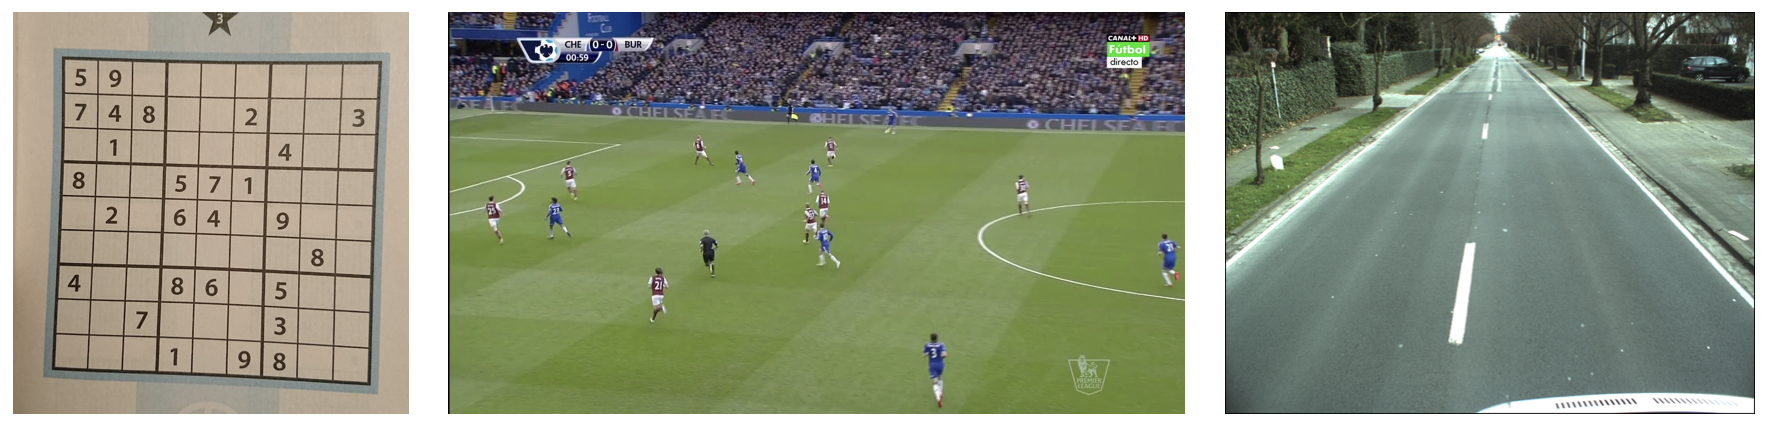
\includegraphics[width=\textwidth]{resources/png/introduction.png}
    \end{figure}
    }
\end{frame}

% ----- Plan of the presentation ----- %
\begin{frame}{Plan of the presentation}
    \tableofcontents
\end{frame}

% ----- Algorithms and main methods ----- %
\section{Algorithms and main methods}

\begin{frame}{Algorithms - Structure of our program}
    \begin{figure}
        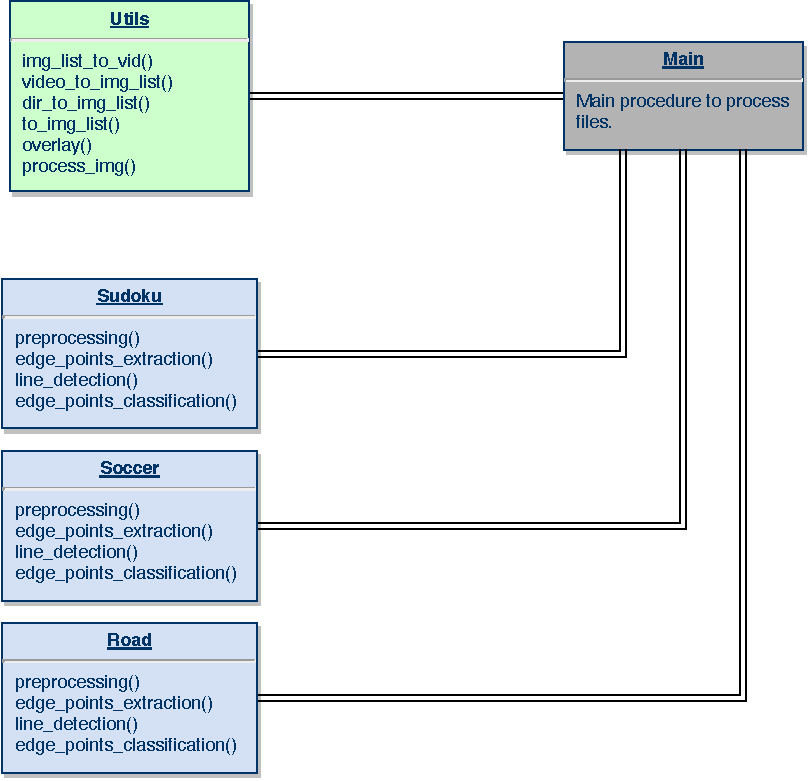
\includegraphics[width=0.7\textwidth]{resources/pdf/uml.pdf}
    \end{figure}
\end{frame}

\begin{frame}{Main methods used}
    Canny's algorithm for \alert{edge extraction}
    \begin{itemize}
        \item Robustness
        \item Not very sensitive to noise
        \item Adaptable
    \end{itemize}
\end{frame}

\begin{frame}{Main methods used}
    Probabilistic Hough transform for \alert{line detection}
    \begin{itemize}
        \item Powerful
        \item Robust to noise
        \item React pretty well to gaps
    \end{itemize}
\end{frame}

% ----- Sudoku images ----- %
\section{Sudoku images}

\begin{frame}{Sudoku procedure}
    \begin{columns}
    \column{0.4\textwidth}
    \begin{enumerate}
        \item<1-> Bilateral filter
        \item<2-> Canny edge detection
        \item<3-> Probabilistic Hough transform, searching for \textbf{long continuous} lines
    \end{enumerate}
    \column{0.3\textwidth}
    \only<1>{
        \begin{figure}
            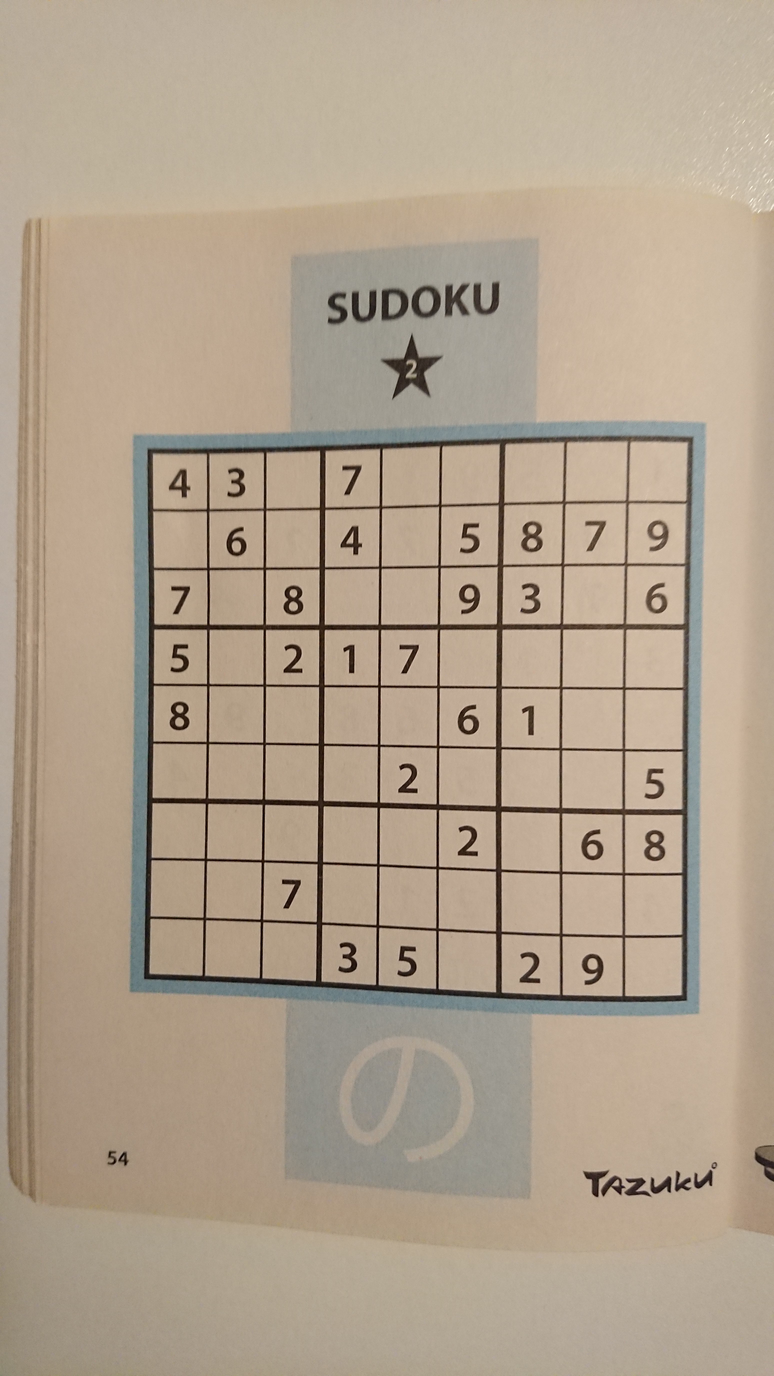
\includegraphics[width=\textwidth]{resources/png/sudoku_00018_00.png}
        \end{figure}
    }
    \only<2>{
        \begin{figure}
            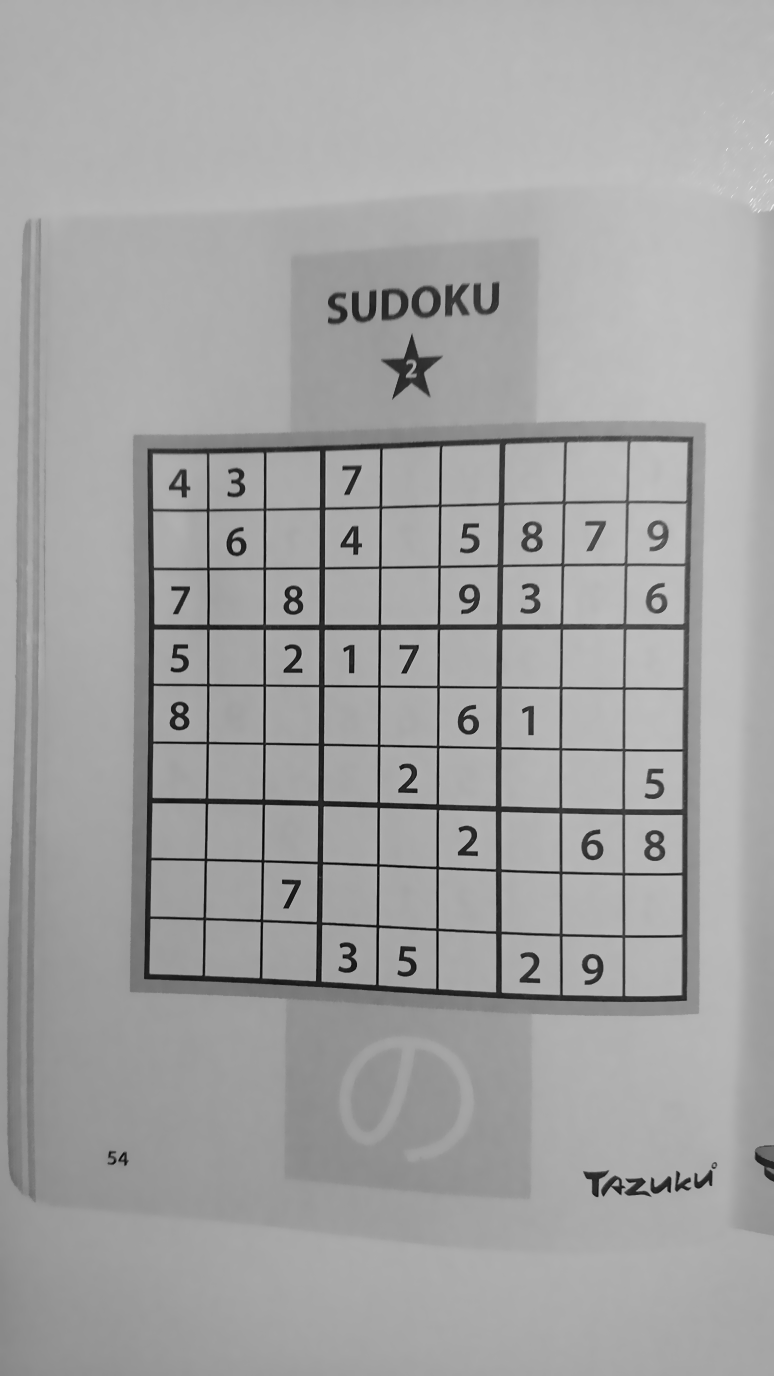
\includegraphics[width=\textwidth]{resources/png/sudoku_00018_01.png}
        \end{figure}
    }
    \only<3->{
        \begin{figure}
            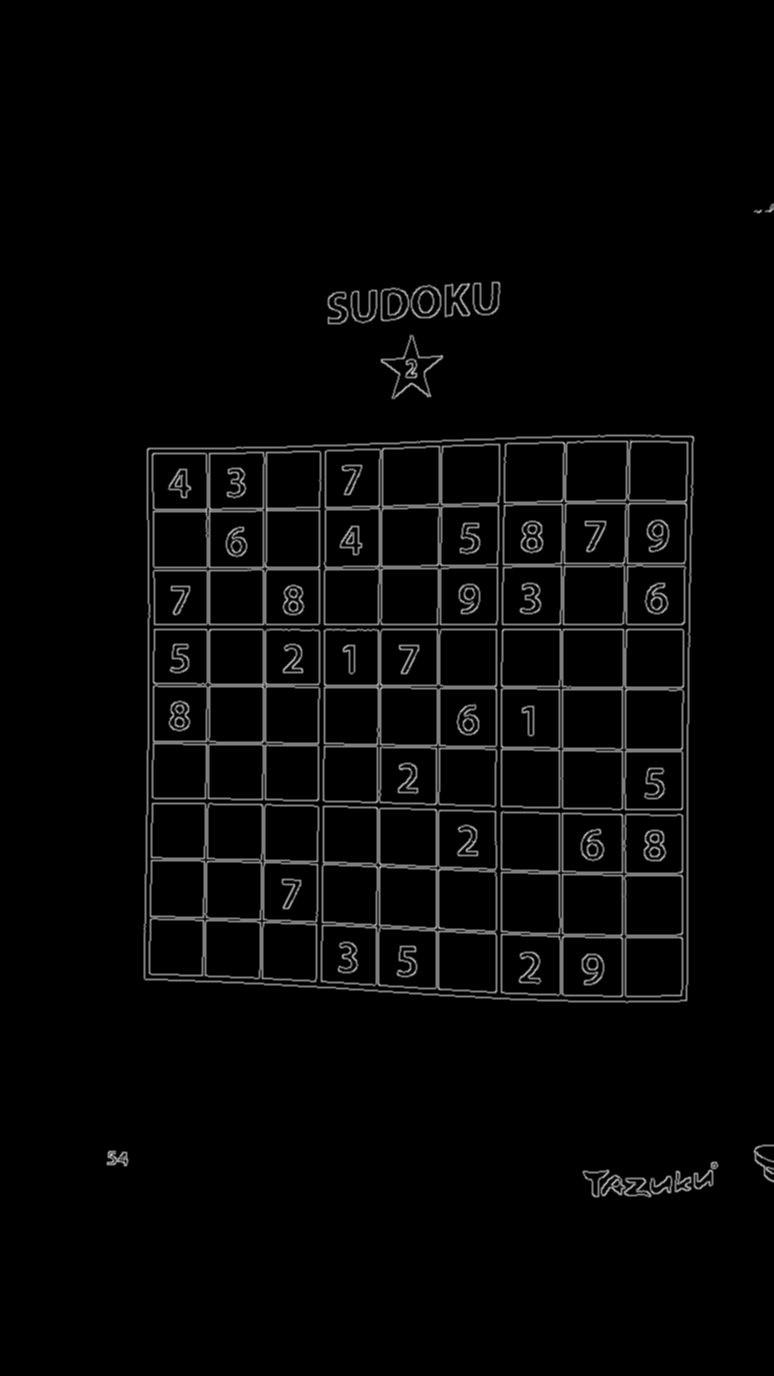
\includegraphics[width=\textwidth]{resources/png/sudoku_00018_02.png}
        \end{figure}
    }
    \column{0.3\textwidth}
    \only<1>{
        \begin{figure}
            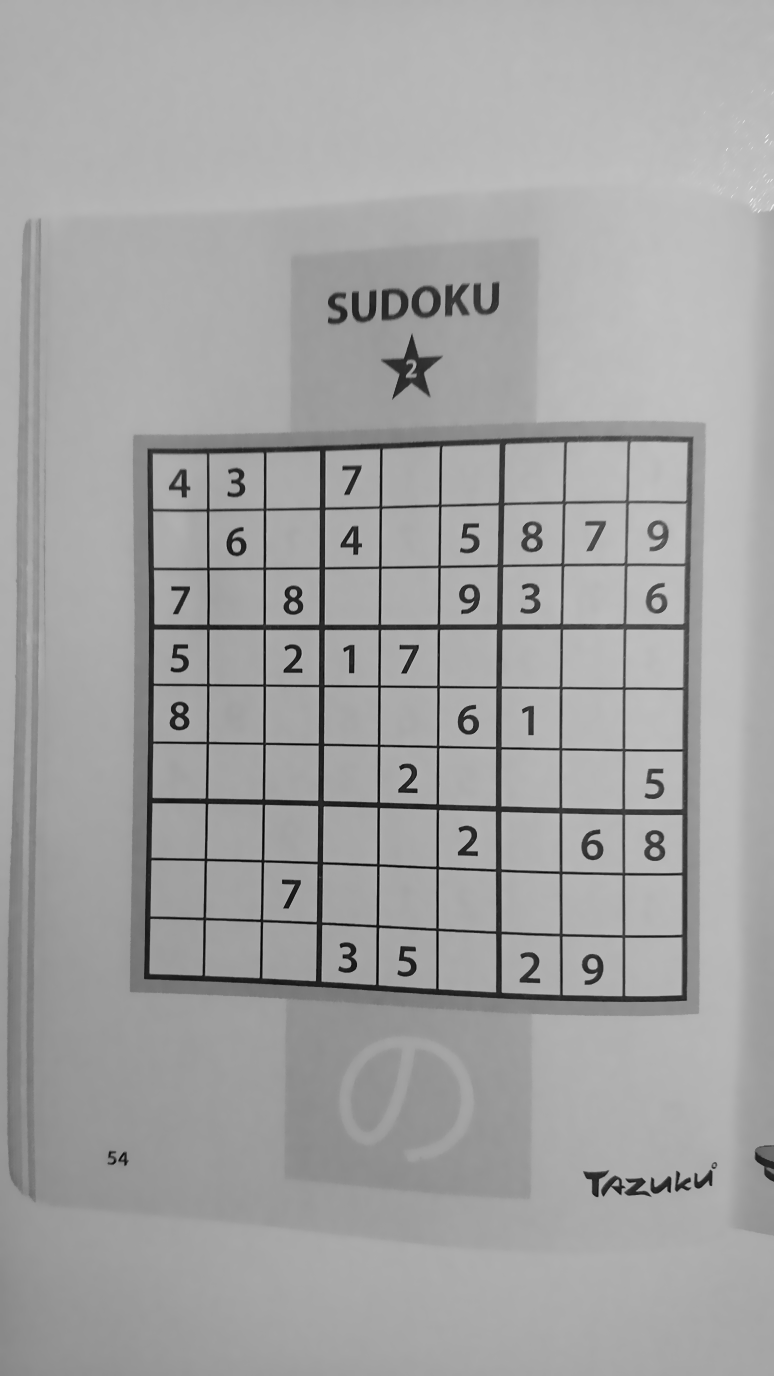
\includegraphics[width=\textwidth]{resources/png/sudoku_00018_01.png}
        \end{figure}
    }
    \only<2>{
        \begin{figure}
            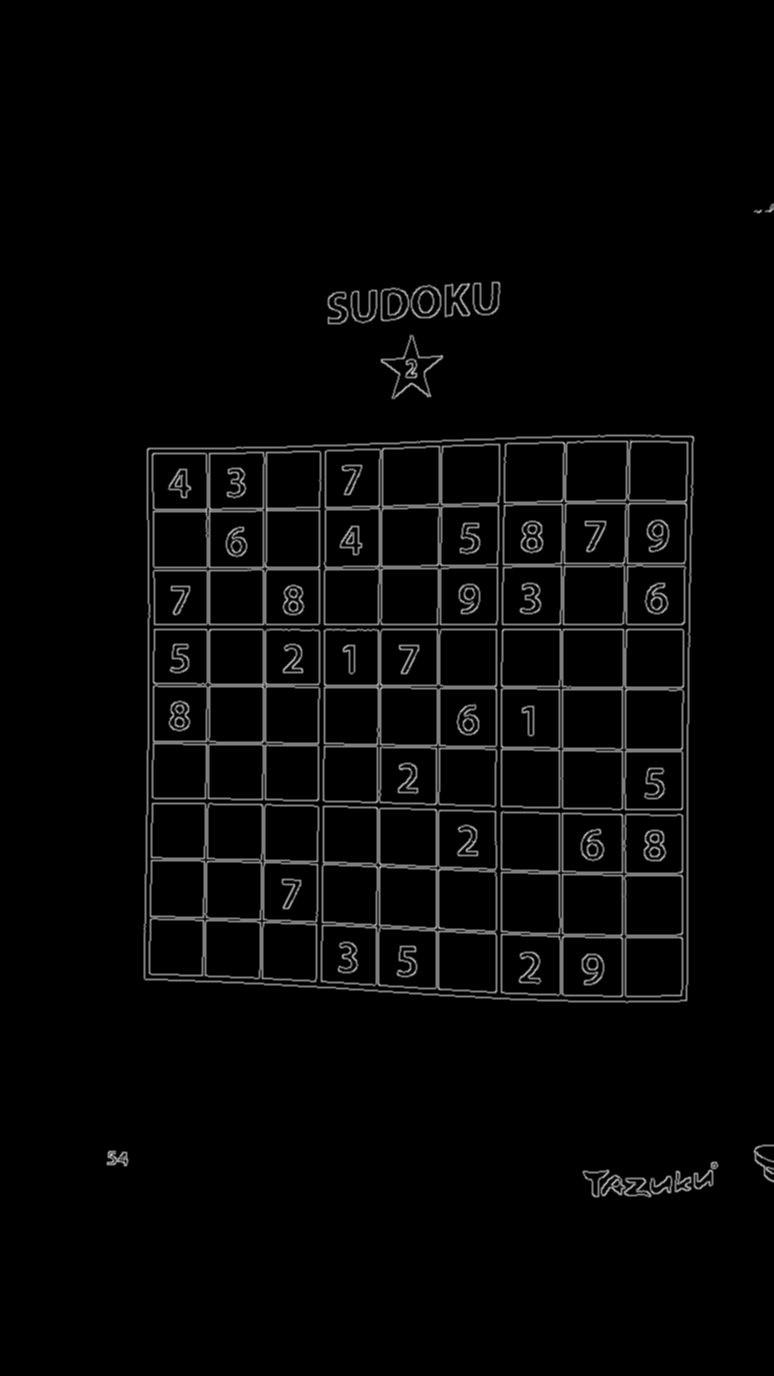
\includegraphics[width=\textwidth]{resources/png/sudoku_00018_02.png}
        \end{figure}
    }
    \only<3->{
        \begin{figure}
            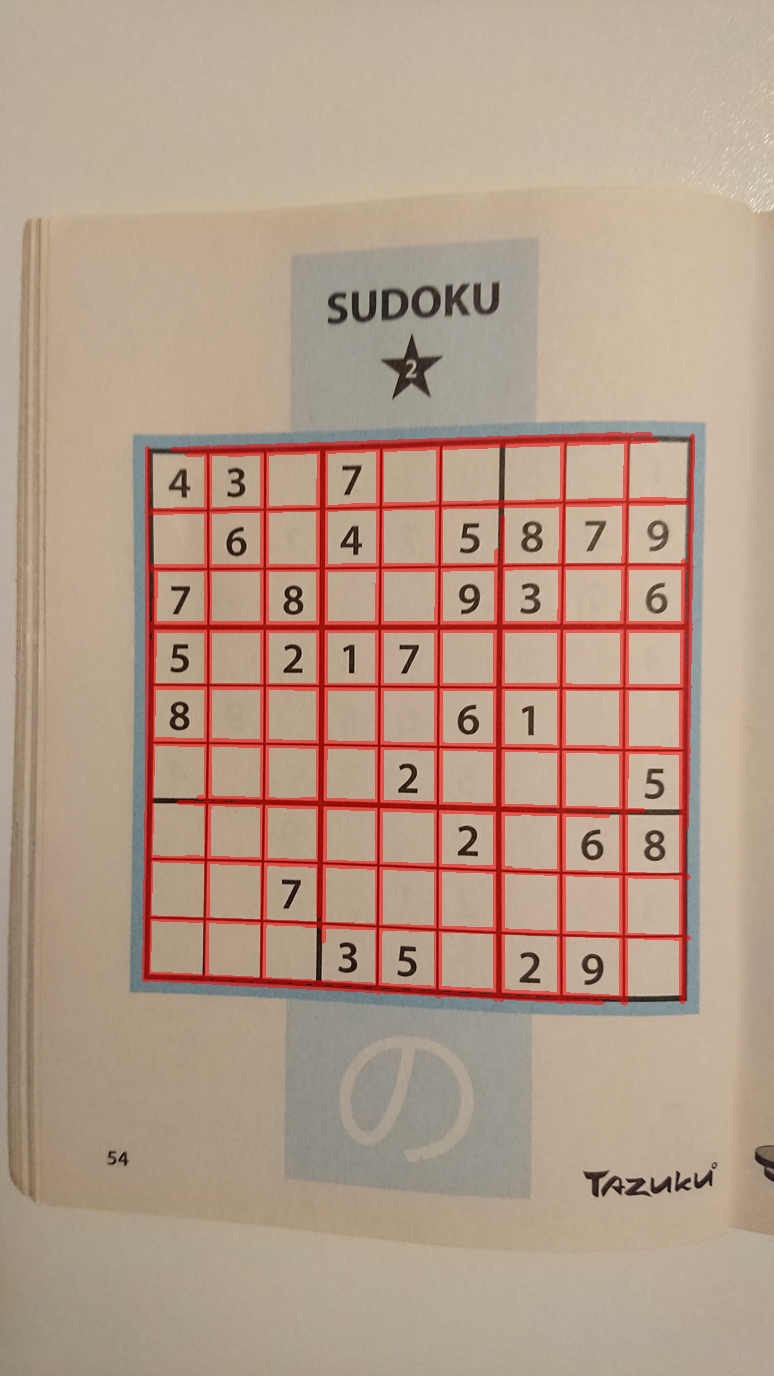
\includegraphics[width=\textwidth]{resources/png/sudoku_00018_04.png}
        \end{figure}
    }
    \end{columns}
\end{frame}

\begin{frame}{Sudoku drawbacks}
    \begin{columns}
        \column{0.6\textwidth}
        Trouble to recognize curved lines.
        \visible<2->{
        \begin{block}{Solutions}
            \begin{itemize}
                \item<2-> Post-processing lines
                \item<3-> Improving \alert{acquisition}
            \end{itemize}
        \end{block}
        }
        \column{0.4\textwidth}
        \begin{figure}
            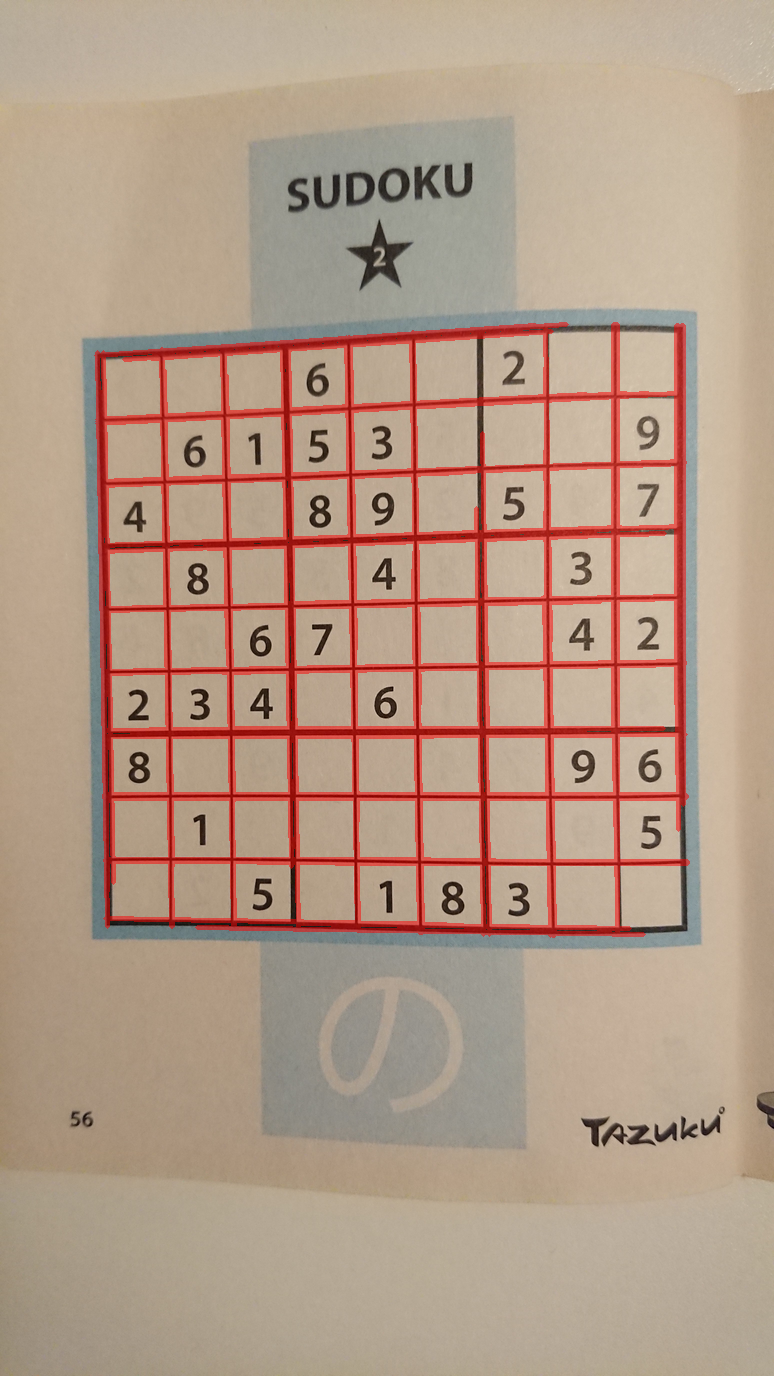
\includegraphics[width=\textwidth]{resources/png/sudoku_00011_04.png}
        \end{figure}
    \end{columns}
\end{frame}

\begin{frame}{Edges classification}
    \begin{columns}
    \column{0.6\textwidth}
    Same procedure for each type of images.
    \begin{enumerate}
        \item Detected lines are traced in white on black image
        \item Edges belonging to white zone are selected
        \item Selected edges are colored in red
    \end{enumerate}
    \column{0.4\textwidth}
    \begin{figure}
        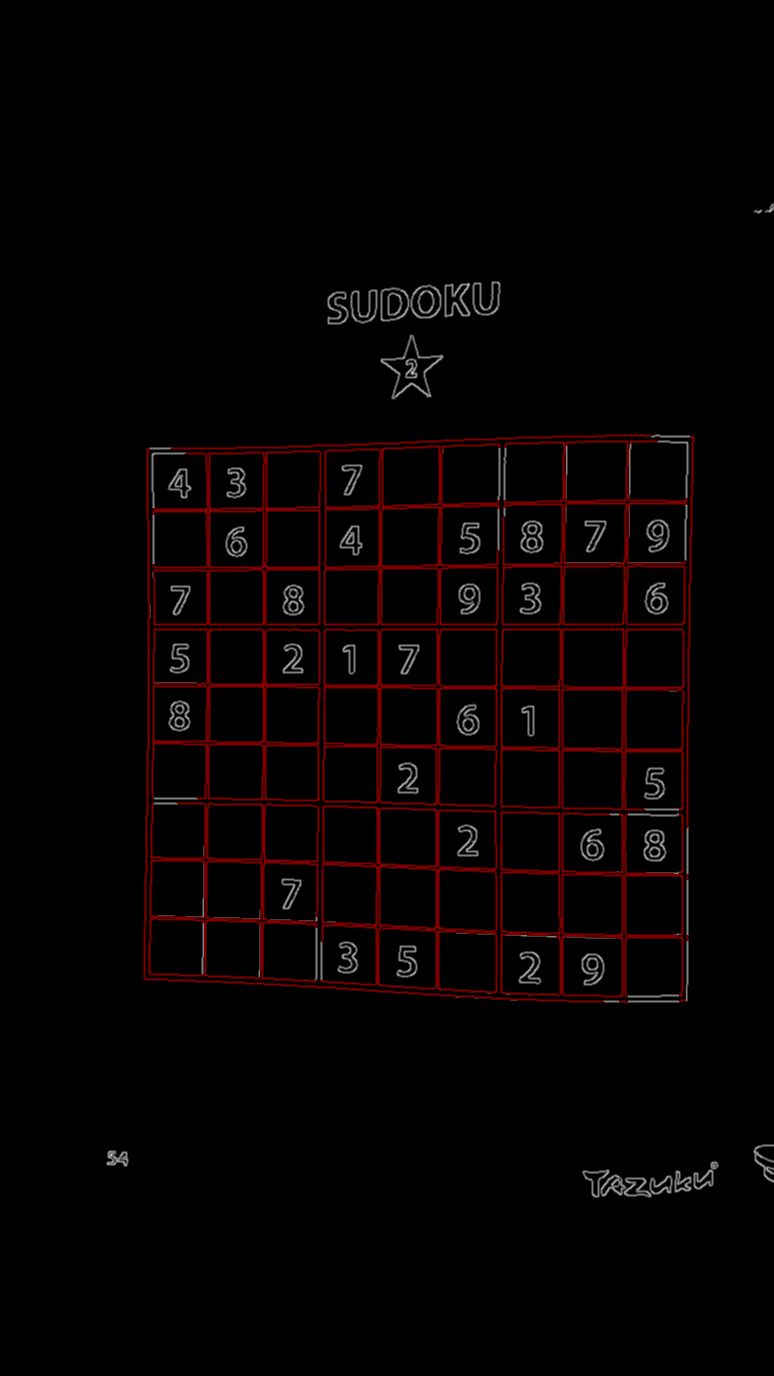
\includegraphics[width=\textwidth]{resources/png/sudoku_00018_03.png}
    \end{figure}
    \end{columns}
\end{frame}

% ----- Soccer images ----- %
\section{Soccer images}

\begin{frame}{Soccer procedure - First try}
    \begin{columns}
    \column{0.4\textwidth}
    \begin{enumerate}
        \item<1-> \alert<4>{Bilateral} filter
        \item<2-> Canny edge detection
        \item<3-> Probabilistic Hough transform, searching for \textbf{long} lines
    \end{enumerate}
    \column{0.6\textwidth}
    \only<1>{
        \begin{figure}
            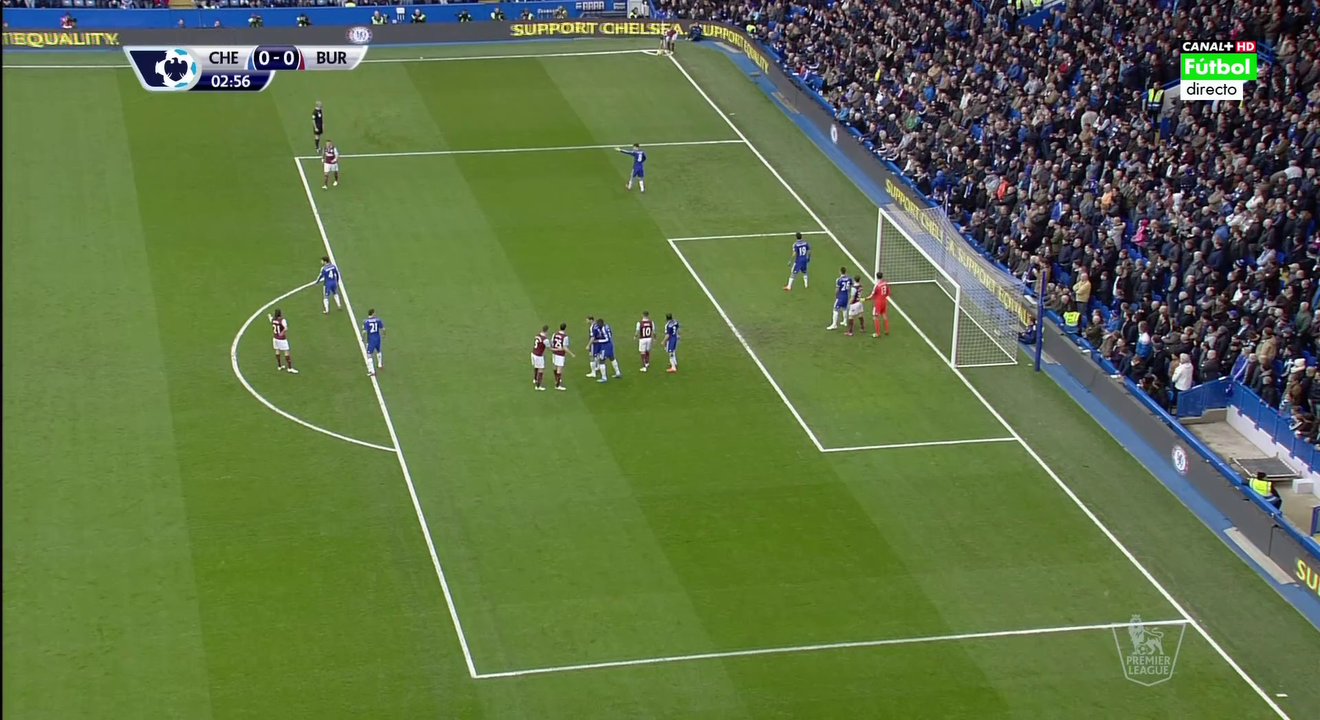
\includegraphics[width=\textwidth]{resources/png/soccer_00020_00_bad.png}
        \end{figure}
        \vspace{-1em}
        \begin{figure}
            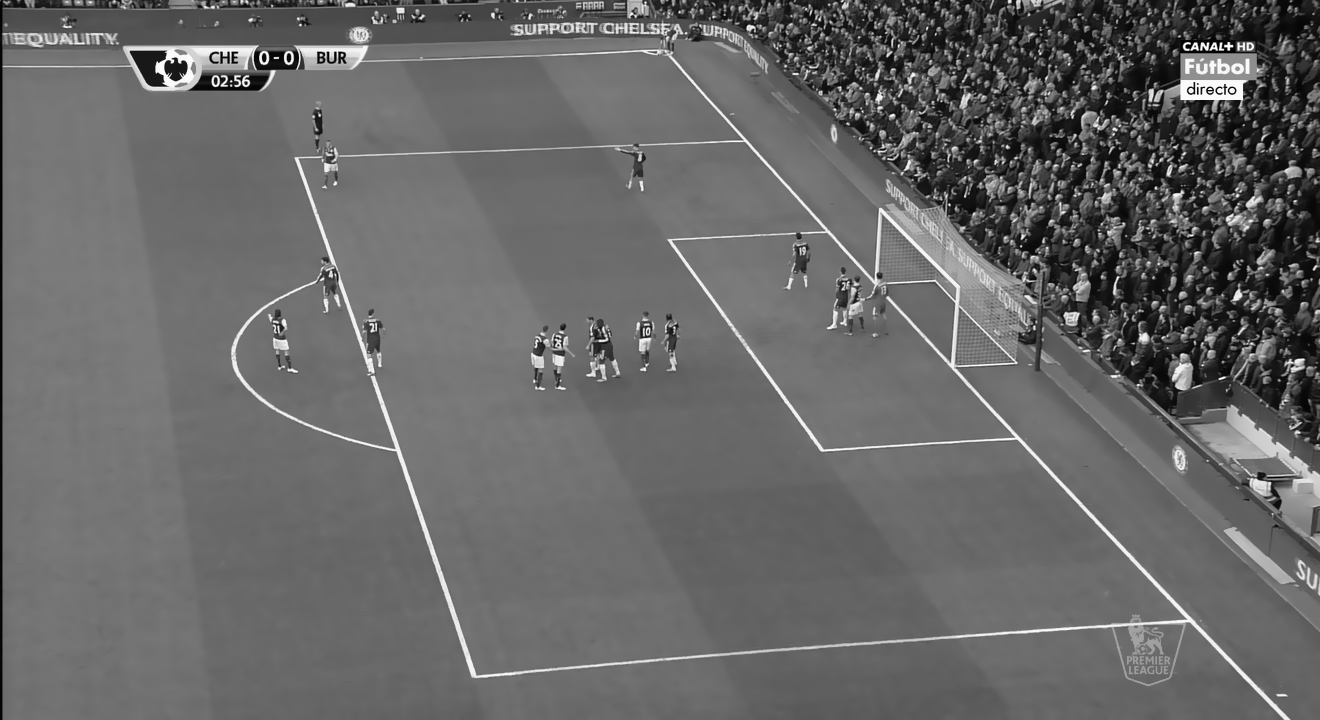
\includegraphics[width=\textwidth]{resources/png/soccer_00020_01_bad.png}
        \end{figure}
    }
    \only<2>{
        \begin{figure}
            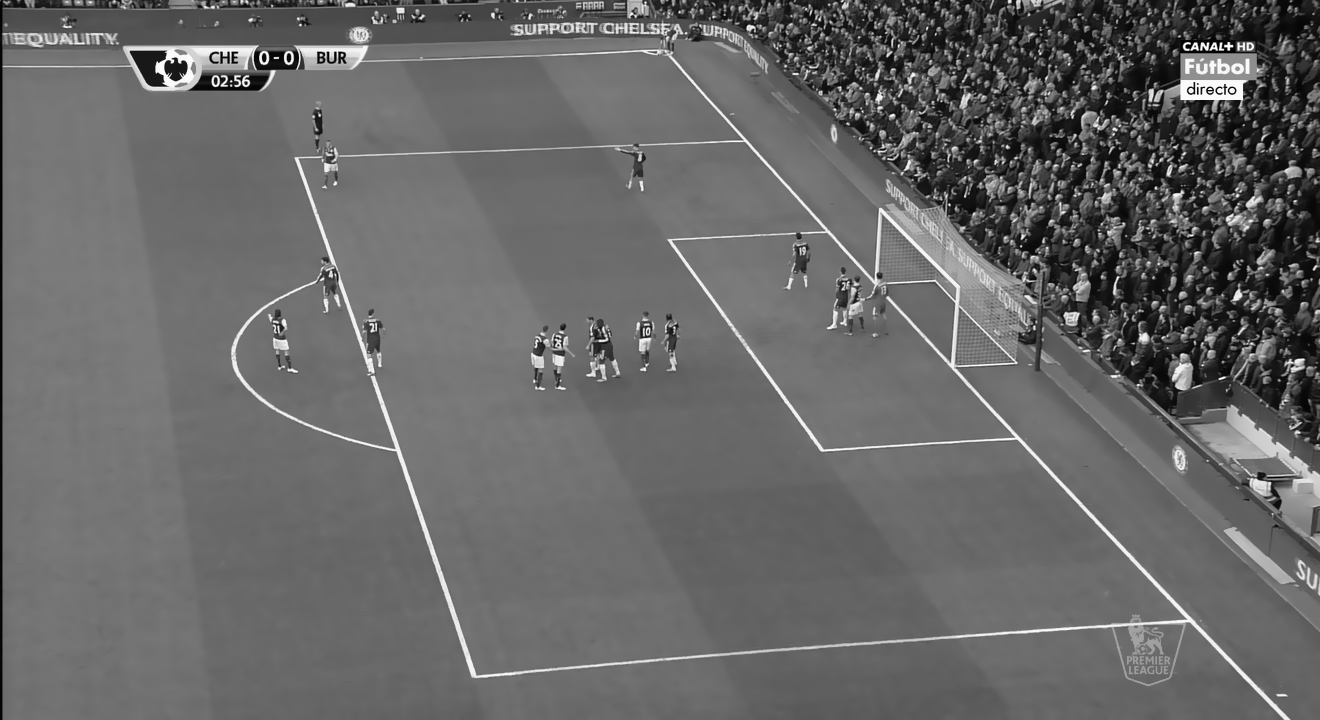
\includegraphics[width=\textwidth]{resources/png/soccer_00020_01_bad.png}
        \end{figure}
        \vspace{-1em}
        \begin{figure}
            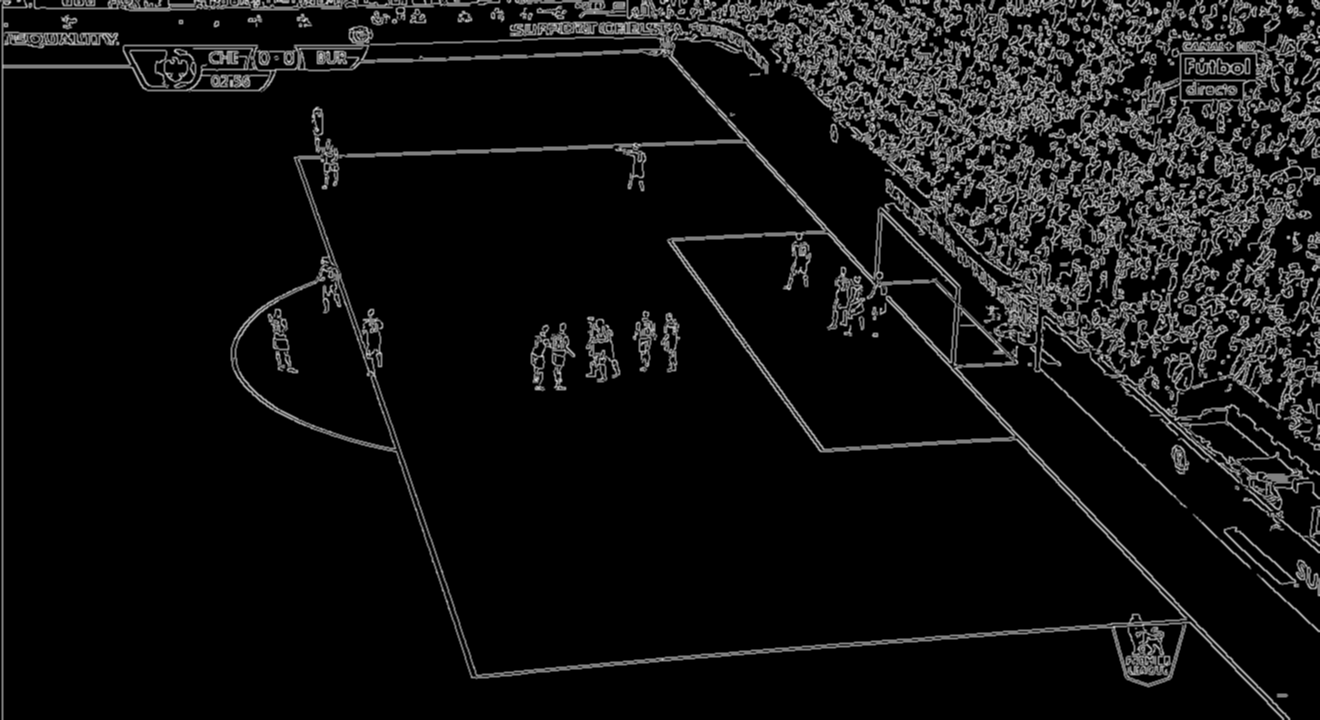
\includegraphics[width=\textwidth]{resources/png/soccer_00020_02_bad.png}
        \end{figure}
    }
    \only<3->{
        \begin{figure}
            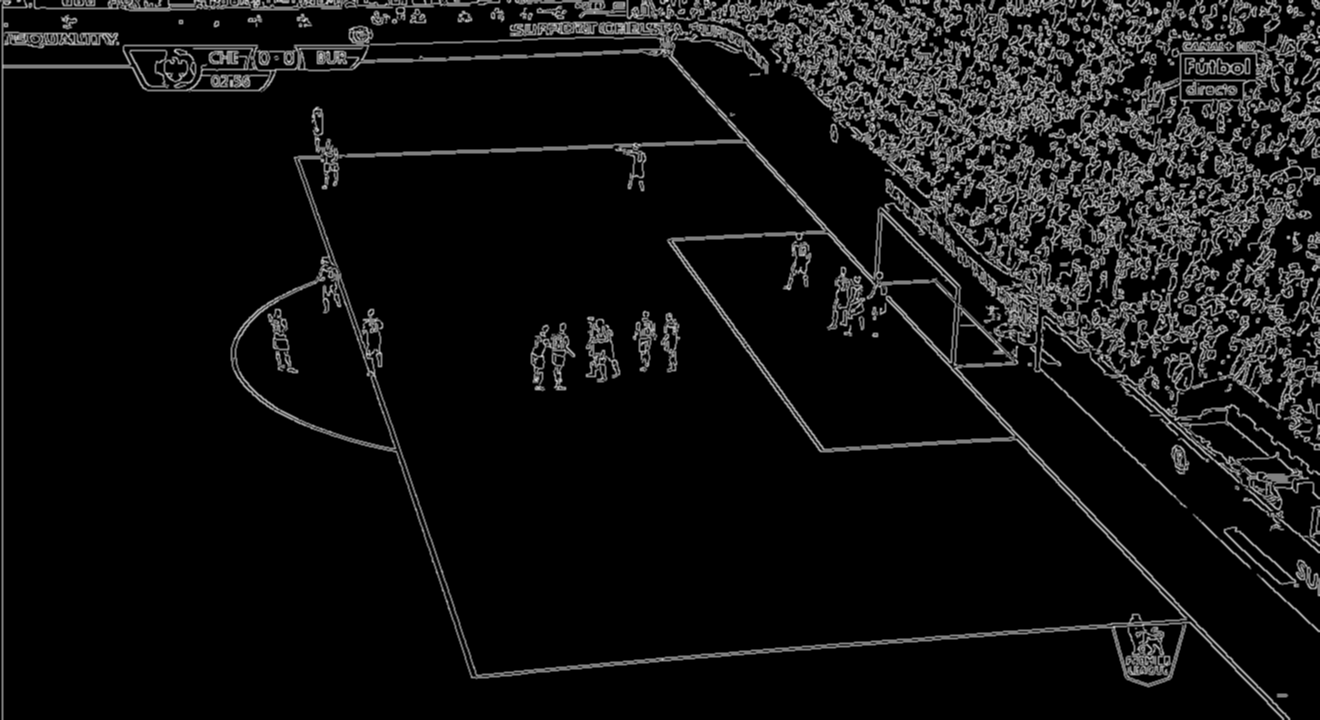
\includegraphics[width=\textwidth]{resources/png/soccer_00020_02_bad.png}
        \end{figure}
        \vspace{-1em}
        \begin{figure}
            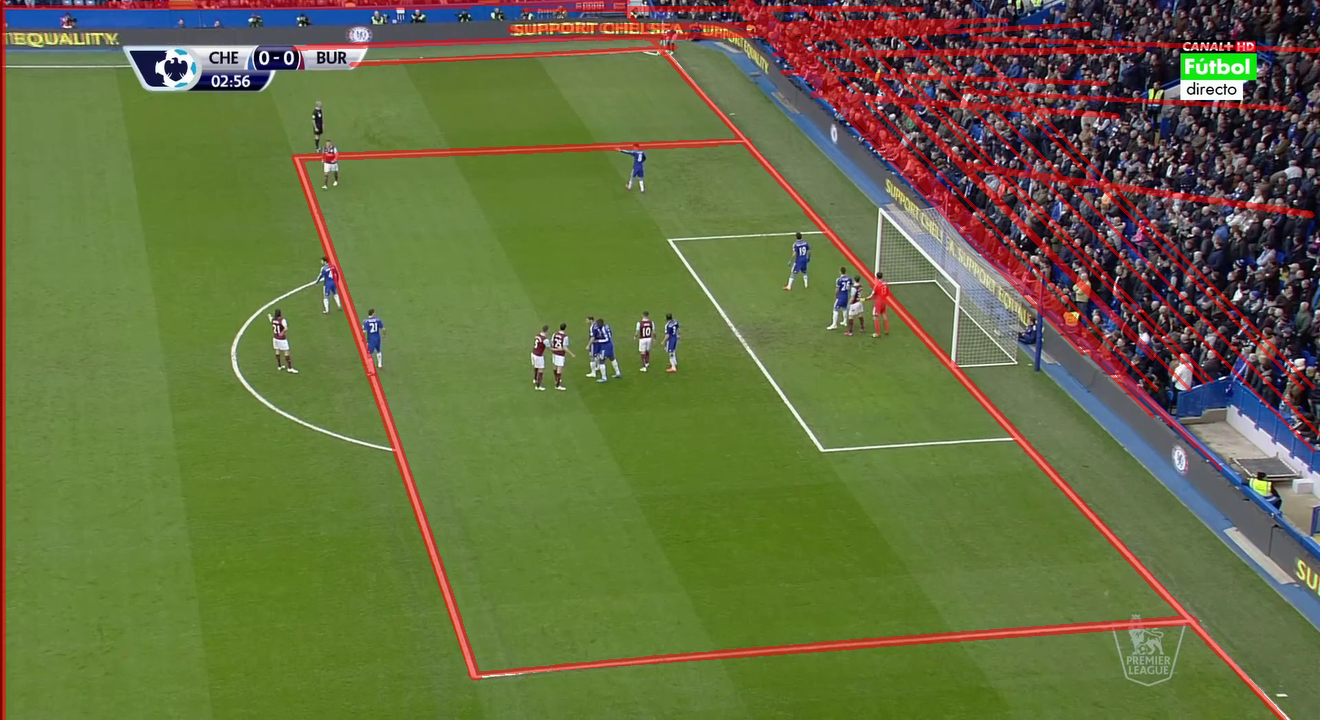
\includegraphics[width=\textwidth]{resources/png/soccer_00020_04_bad.png}
        \end{figure}
    }
    \end{columns}
\end{frame}

\begin{frame}{Soccer procedure - Second try}
    \begin{columns}
    \column{0.4\textwidth}
    \begin{enumerate}
        \item<1-> \textcolor<4>{mLightGreen}{Hue} filter
        \item<2-> Canny edge detection
        \item<3-> Probabilistic Hough transform, searching for \textbf{long} lines
    \end{enumerate}
    \column{0.6\textwidth}
    \only<1>{
        \begin{figure}
            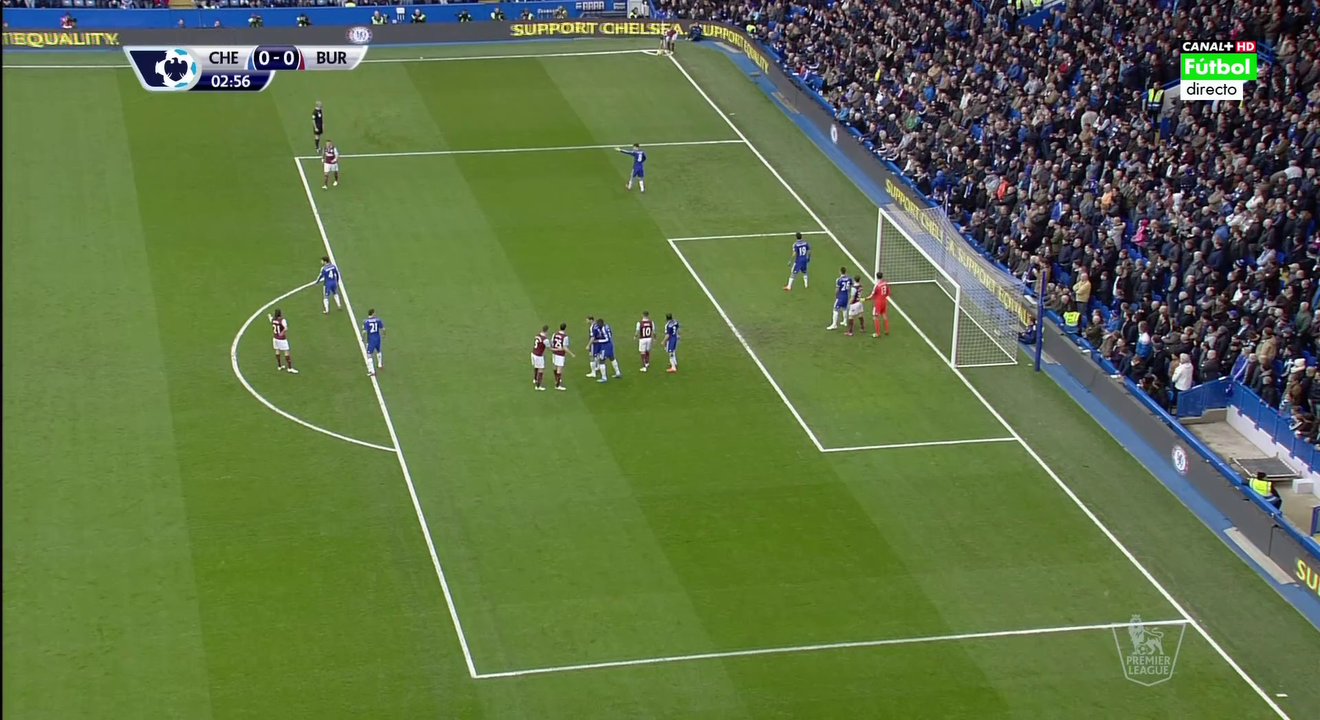
\includegraphics[width=\textwidth]{resources/png/soccer_00020_00.png}
        \end{figure}
        \vspace{-1em}
        \begin{figure}
            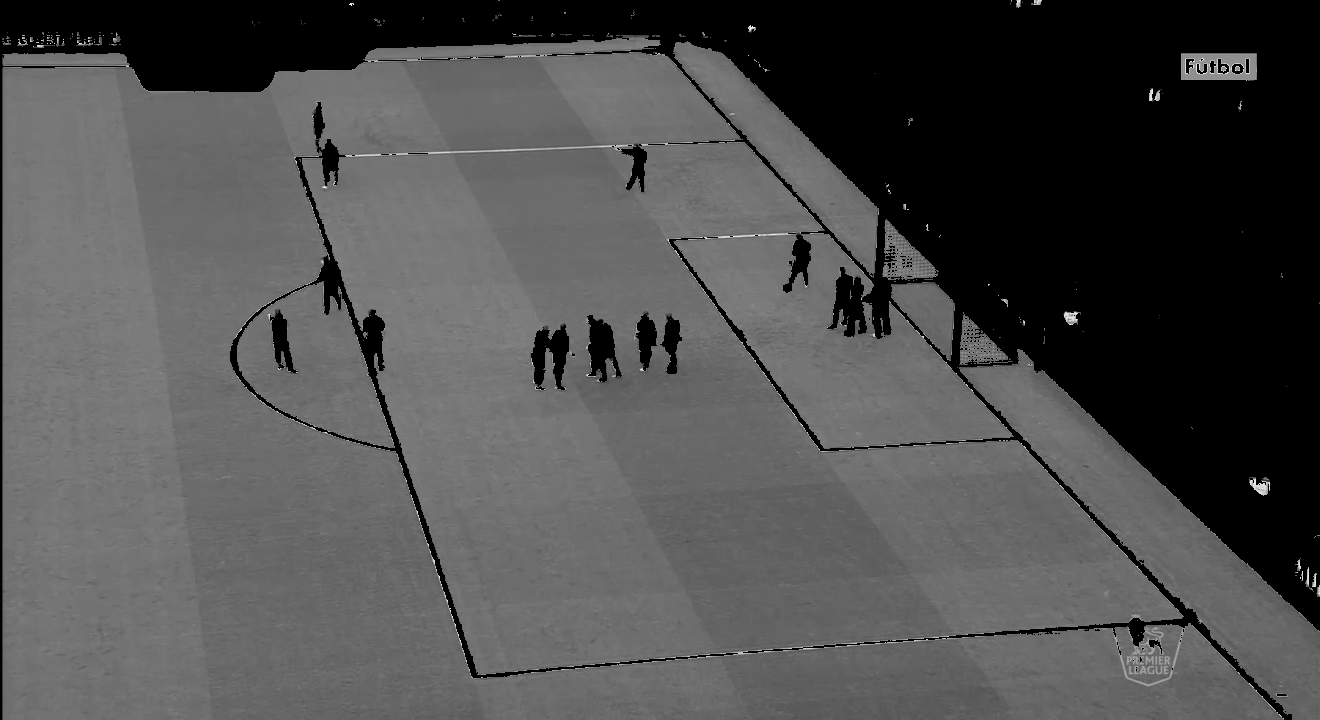
\includegraphics[width=\textwidth]{resources/png/soccer_00020_01.png}
        \end{figure}
    }
    \only<2>{
        \begin{figure}
            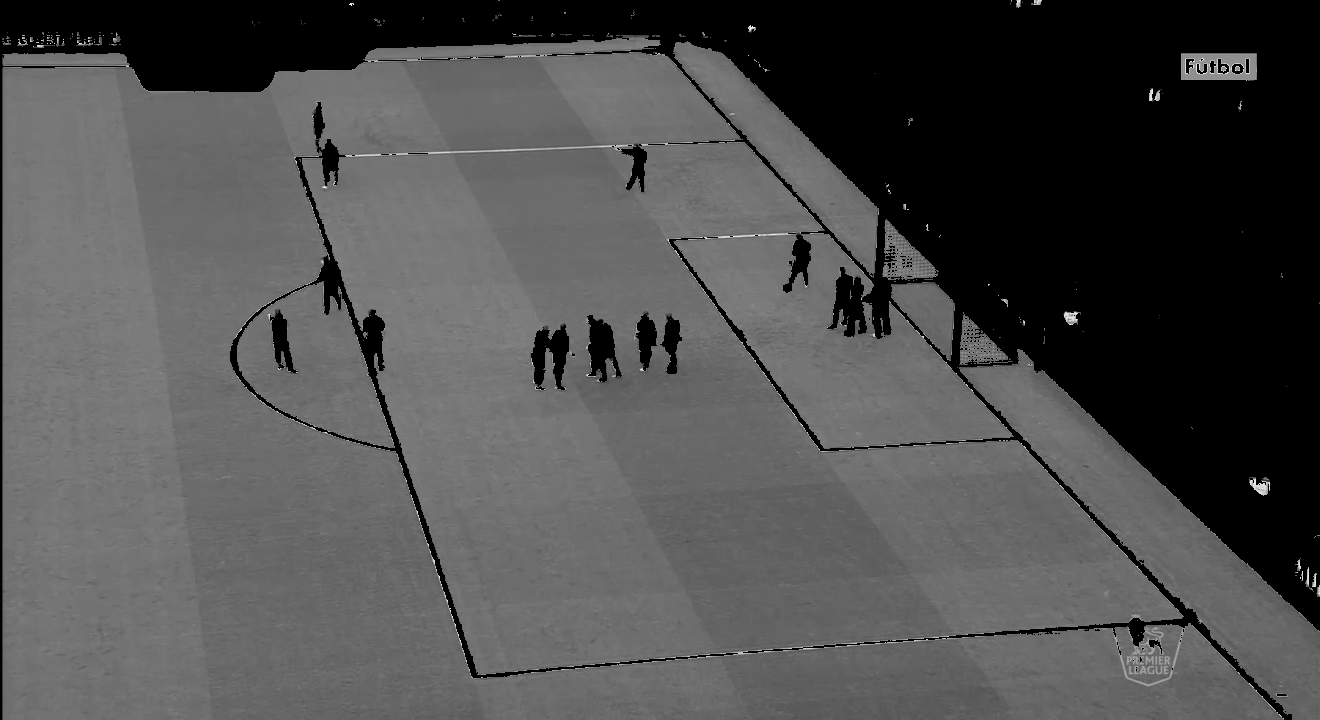
\includegraphics[width=\textwidth]{resources/png/soccer_00020_01.png}
        \end{figure}
        \vspace{-1em}
        \begin{figure}
            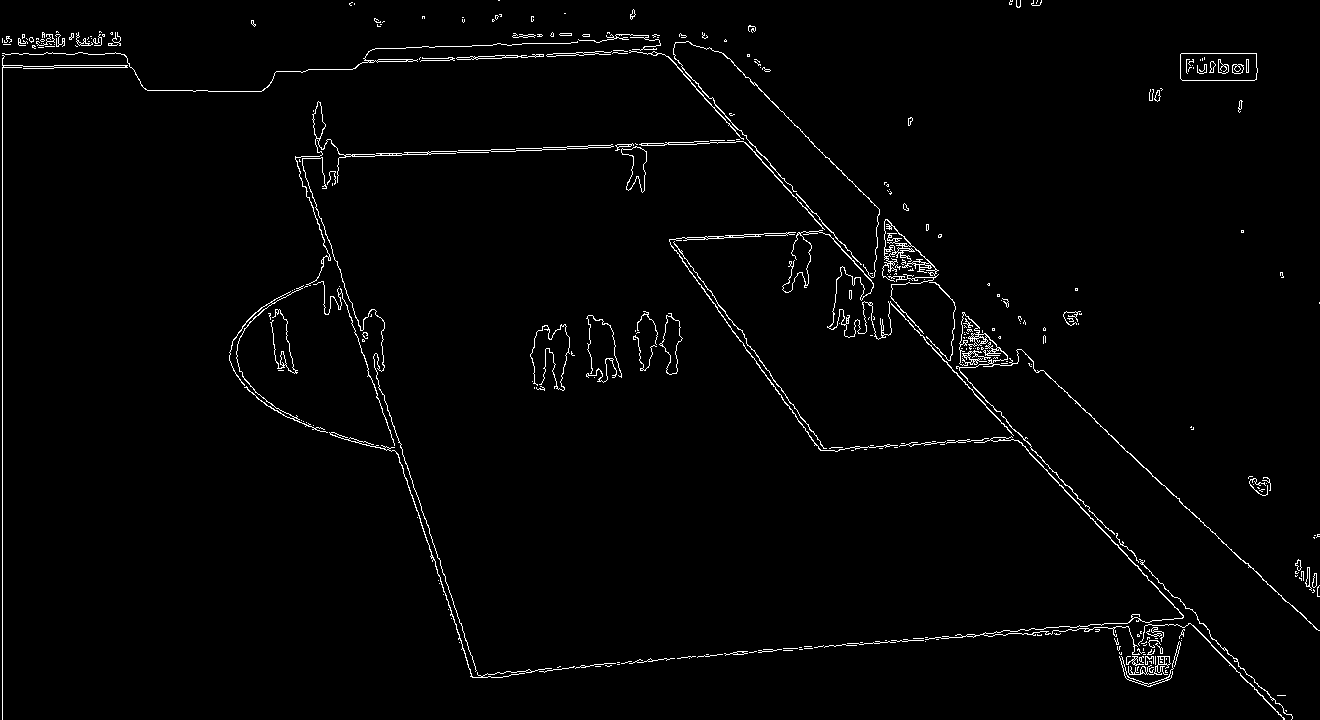
\includegraphics[width=\textwidth]{resources/png/soccer_00020_02.png}
        \end{figure}
    }
    \only<3->{
        \begin{figure}
            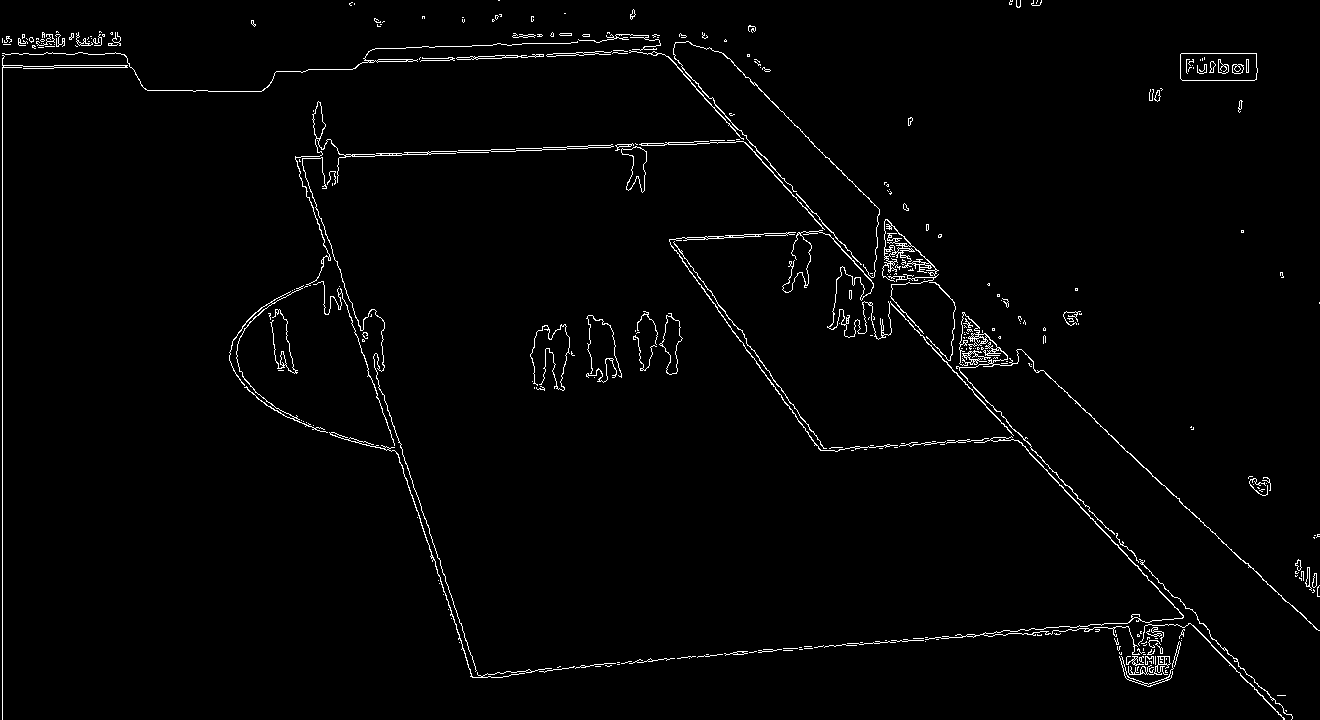
\includegraphics[width=\textwidth]{resources/png/soccer_00020_02.png}
        \end{figure}
        \vspace{-1em}
        \begin{figure}
            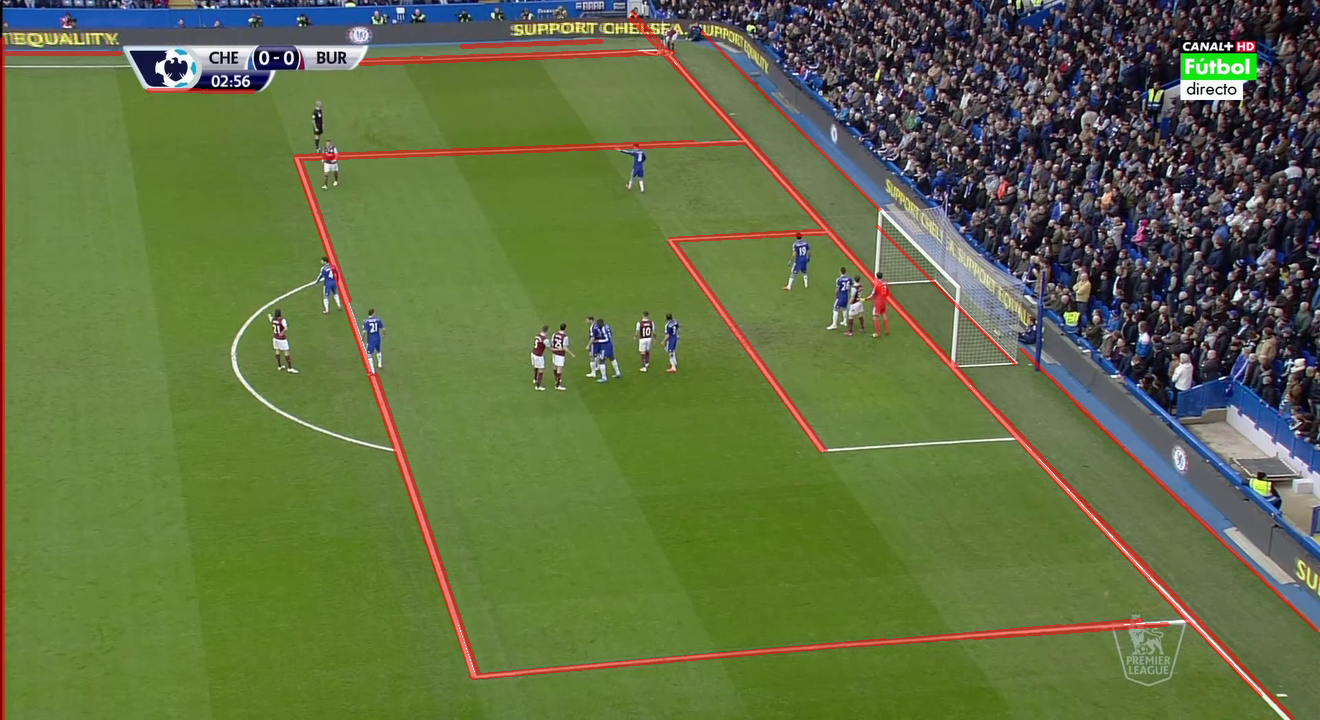
\includegraphics[width=\textwidth]{resources/png/soccer_00020_04.png}
        \end{figure}
    }
    \end{columns}
\end{frame}

% ----- Road images ----- %
\section{Road images}

\begin{frame}{Road procedure}
    \begin{columns}
    \column{0.55\textwidth}
    \begin{enumerate}
        \item<1-> Filter the white components
        \item<2-> Remove big white areas (findContours)
        \item<3-> Canny edge detection
        \item<4-> Probabilistic Hough
    \end{enumerate}
    \column{0.45\textwidth}
    \only<1>{ 
        \begin{figure}
            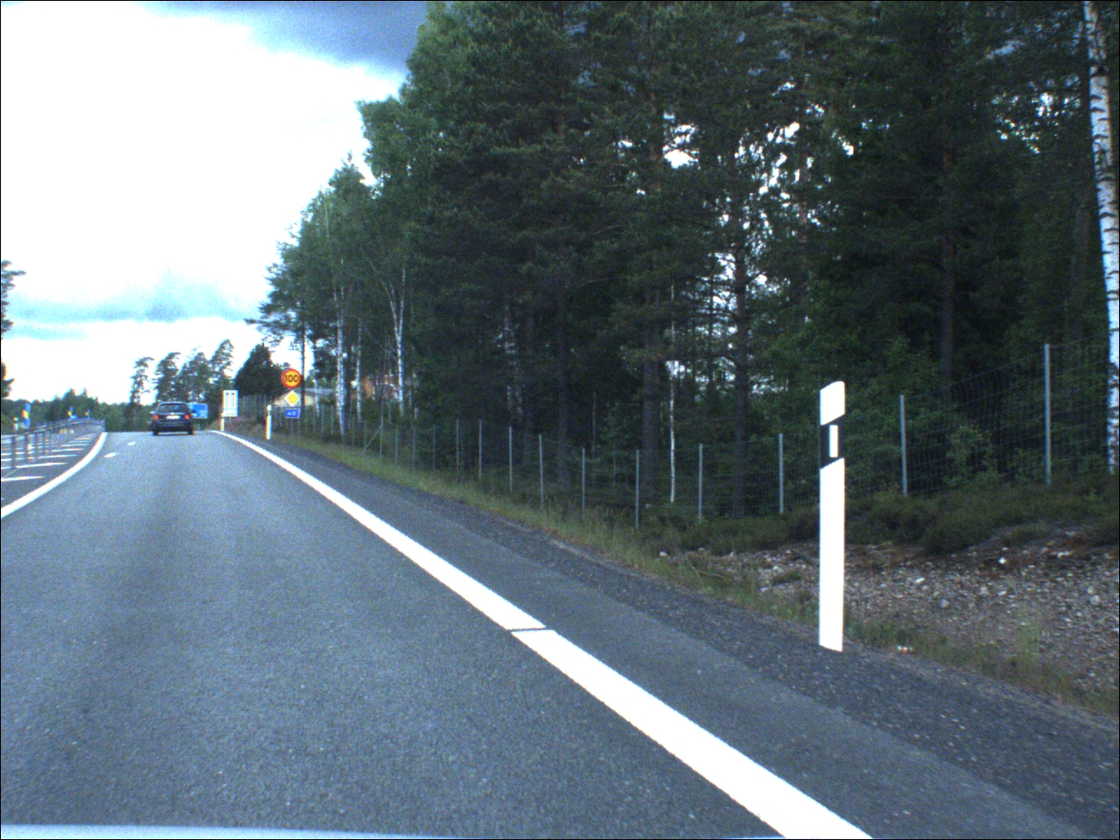
\includegraphics[width=\textwidth]{resources/png/road1.png}
        \end{figure}
        \vspace{-1.3em}
        \begin{figure}
            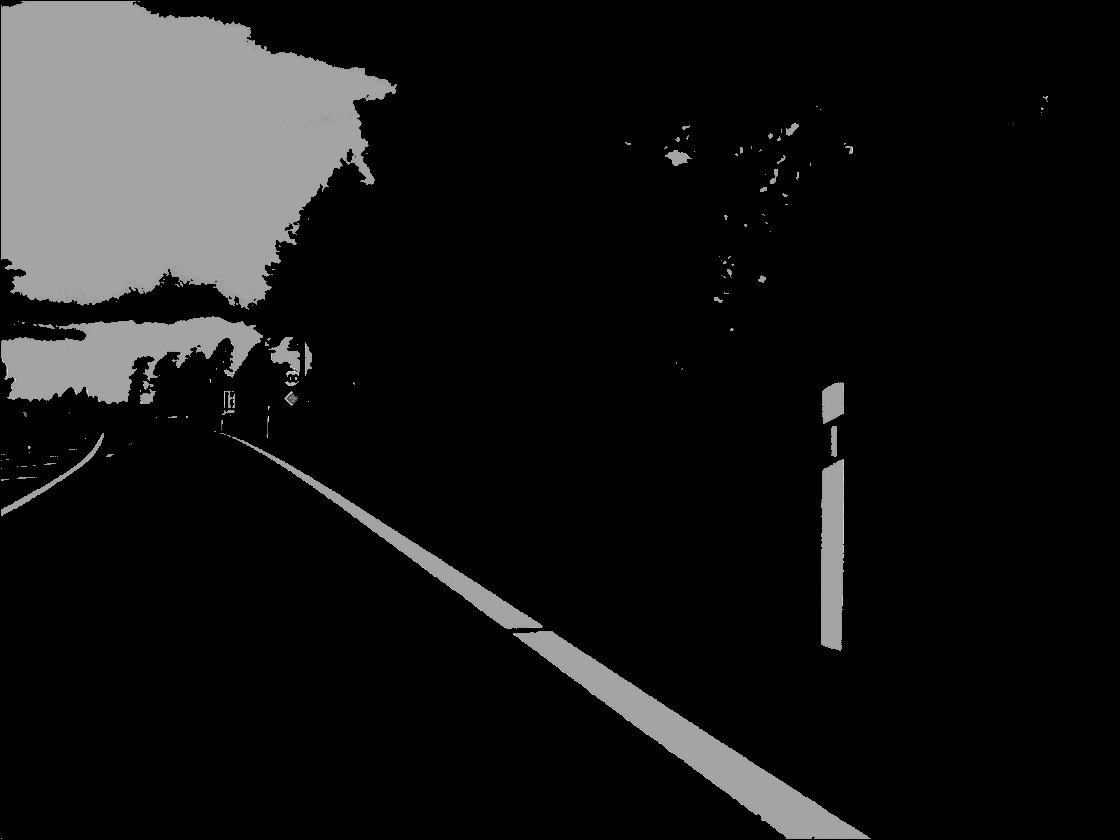
\includegraphics[width=\textwidth]{resources/png/roadwhite.png}
        \end{figure}
    }
    \only<2>{
        \begin{figure}
            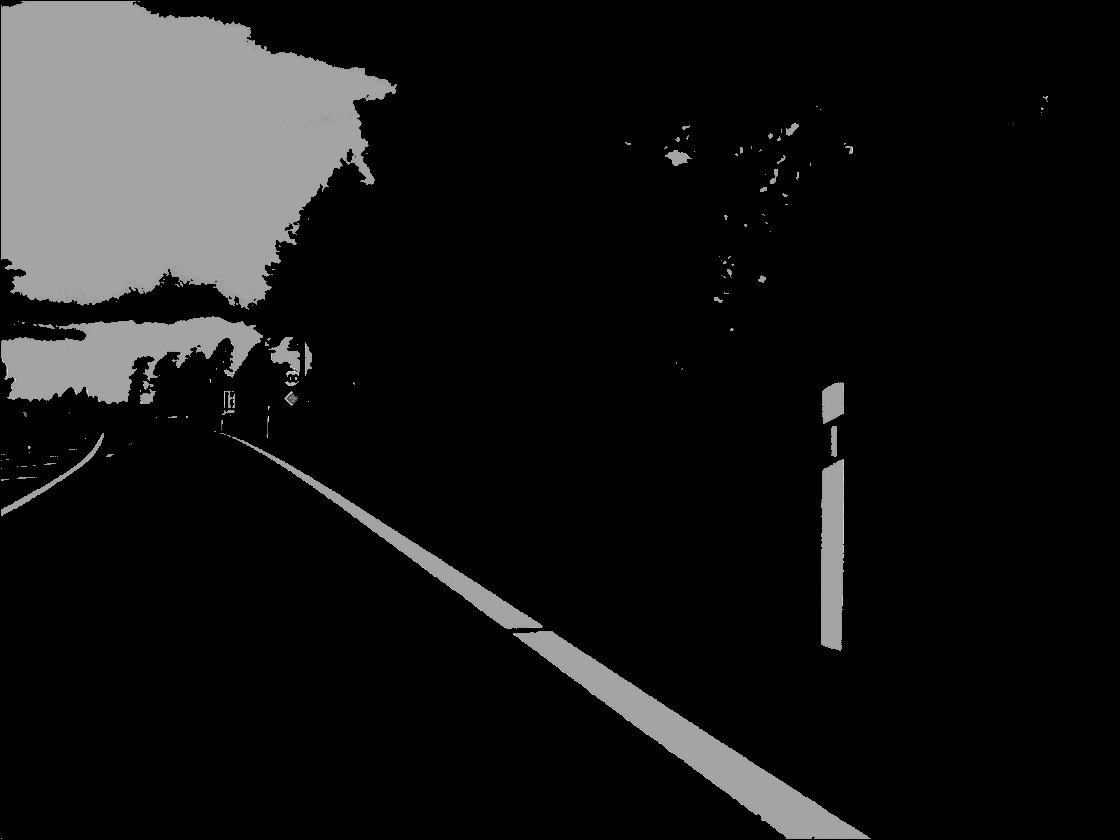
\includegraphics[width=\textwidth]{resources/png/roadwhite.png}
        \end{figure}
        \vspace{-1.3em}
        \begin{figure}
            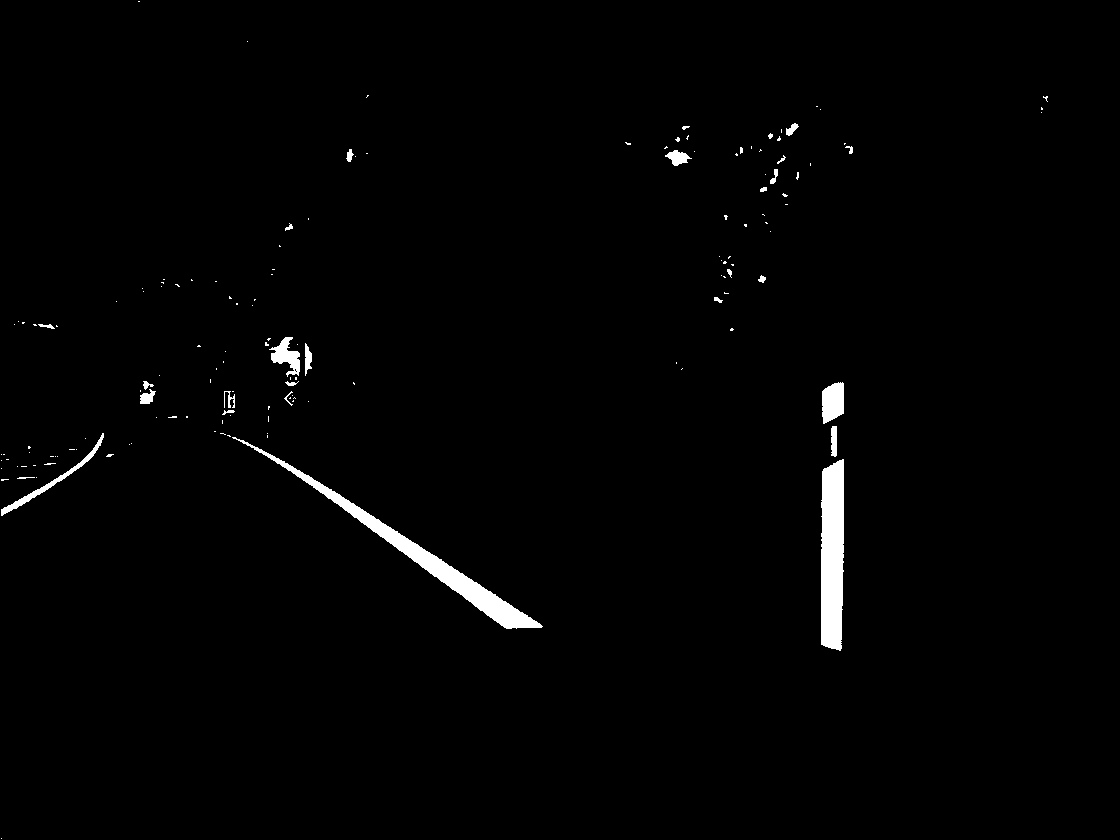
\includegraphics[width=\textwidth]{resources/png/roadnosky.png}
        \end{figure}
    }
    \only<3>{
        \begin{figure}
            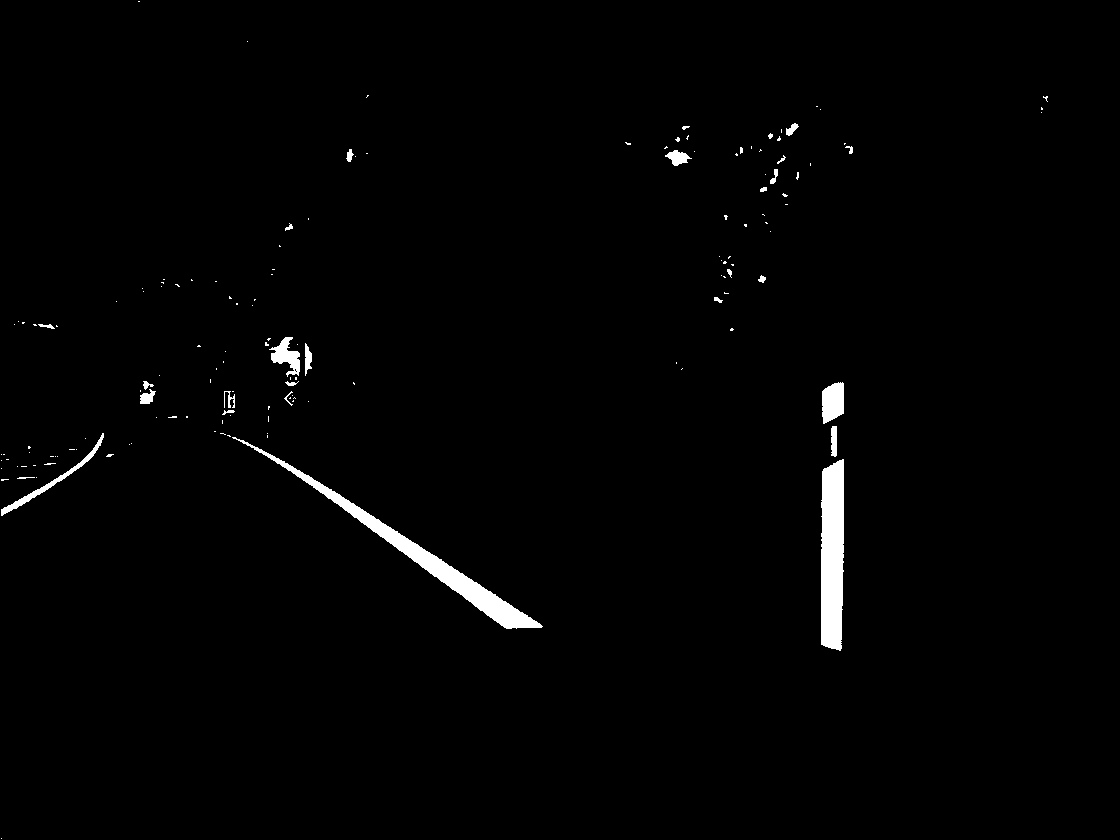
\includegraphics[width=\textwidth]{resources/png/roadnosky.png}
        \end{figure}
        \vspace{-1.3em}
        \begin{figure}
            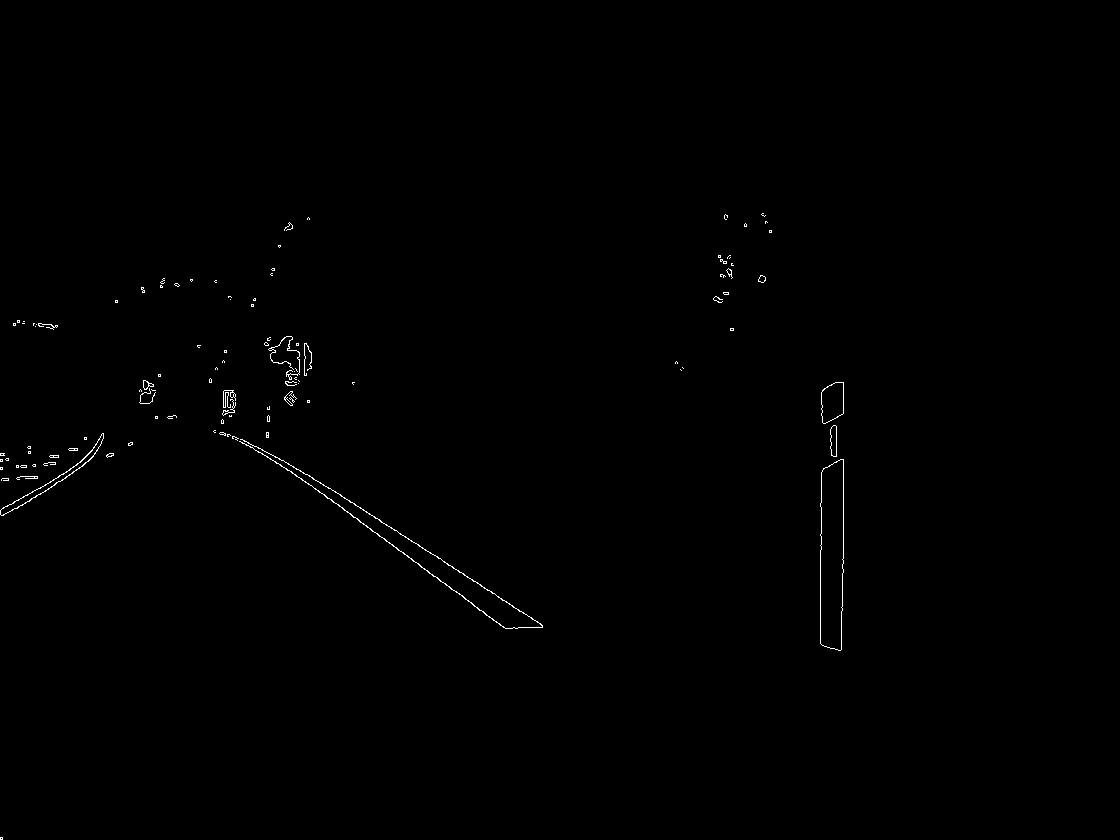
\includegraphics[width=\textwidth]{resources/png/roadcanny.png}
        \end{figure}
    }
    \only<4>{
        \begin{figure}
            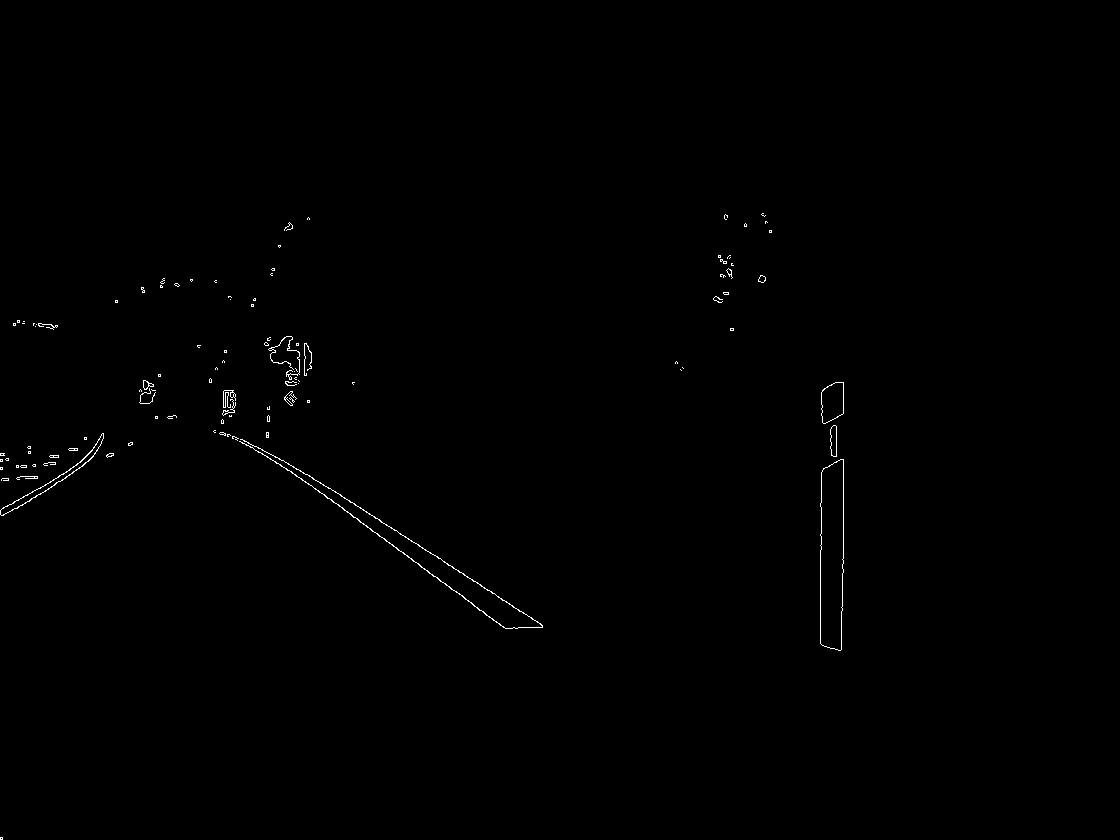
\includegraphics[width=\textwidth]{resources/png/roadcanny.png}
        \end{figure}
        \vspace{-1.3em}
        \begin{figure}
            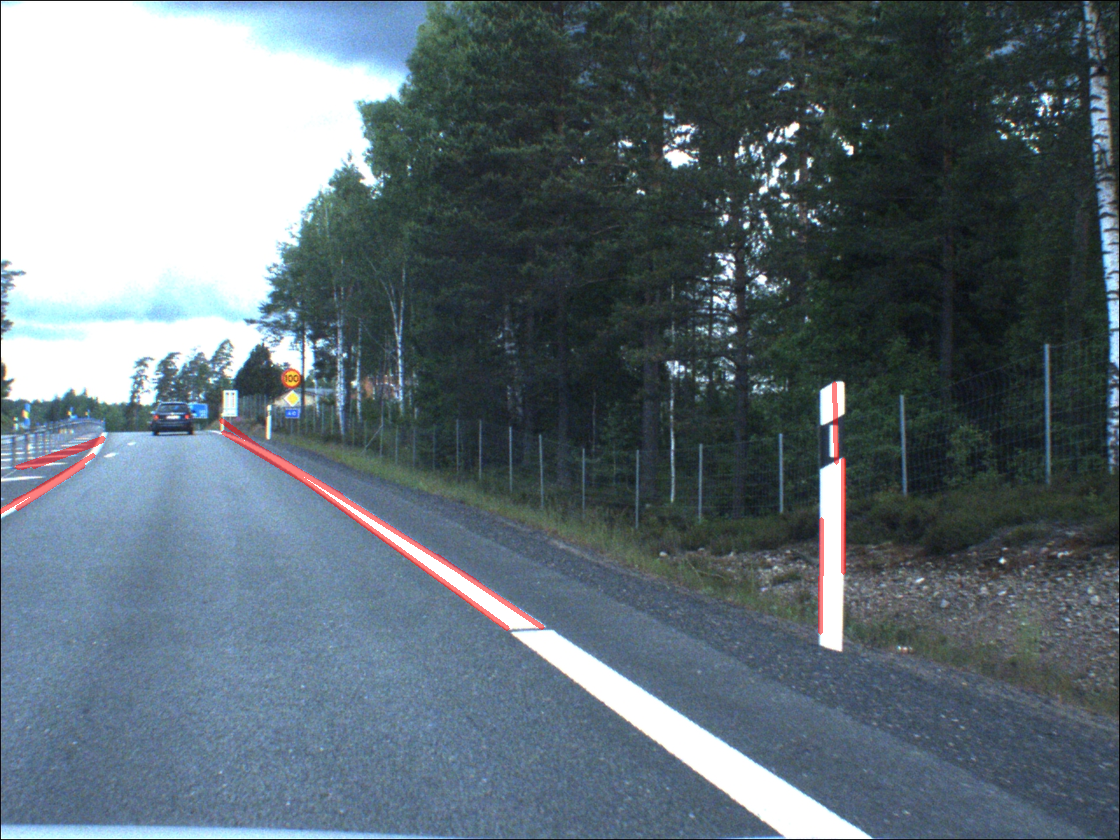
\includegraphics[width=\textwidth]{resources/png/roadhough.png}
        \end{figure}
    }
    \end{columns}
\end{frame}

\begin{frame}{Road discussion}
    \begin{figure}
        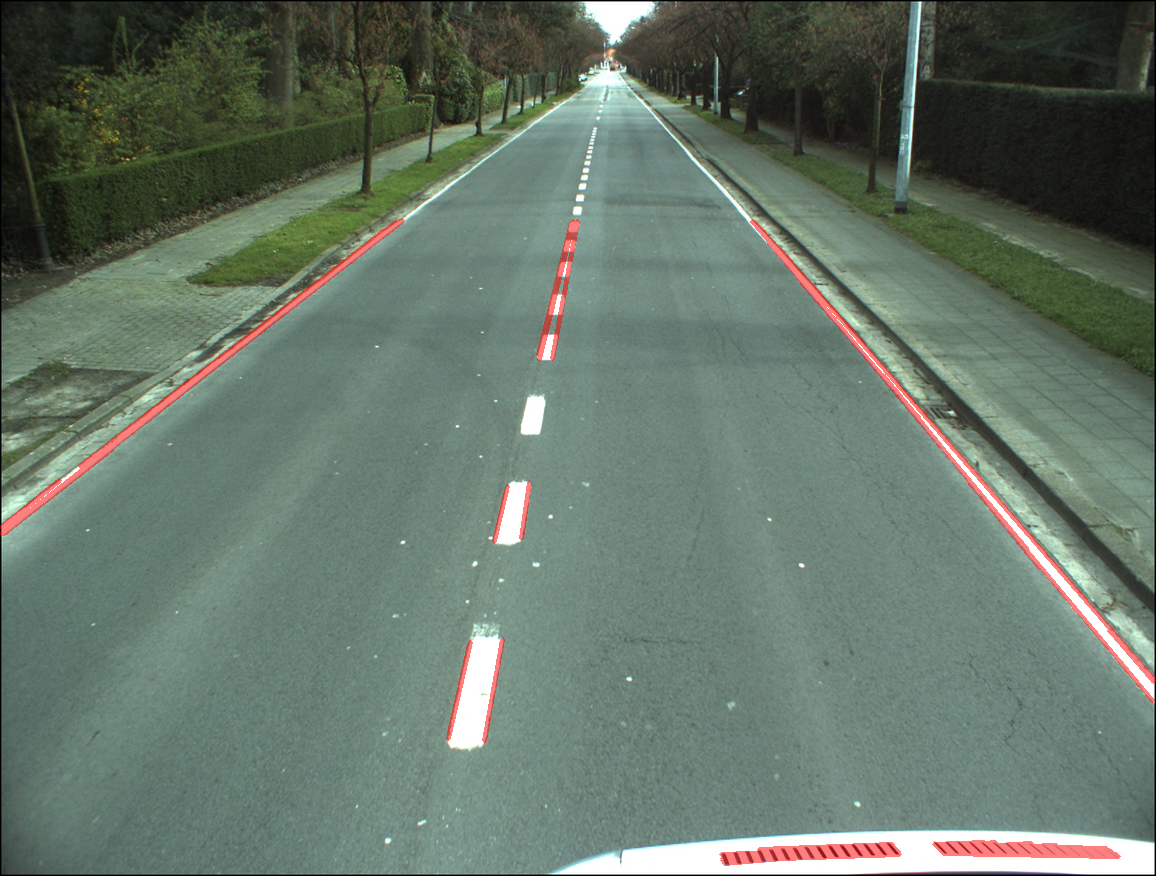
\includegraphics[width=0.9\textwidth]{resources/png/roadgood.png}
    \end{figure}
\end{frame}

\begin{frame}{Road discussion - Imperfect algorithm}
    \begin{columns}
        \column{0.45\textwidth}
        \begin{figure}
            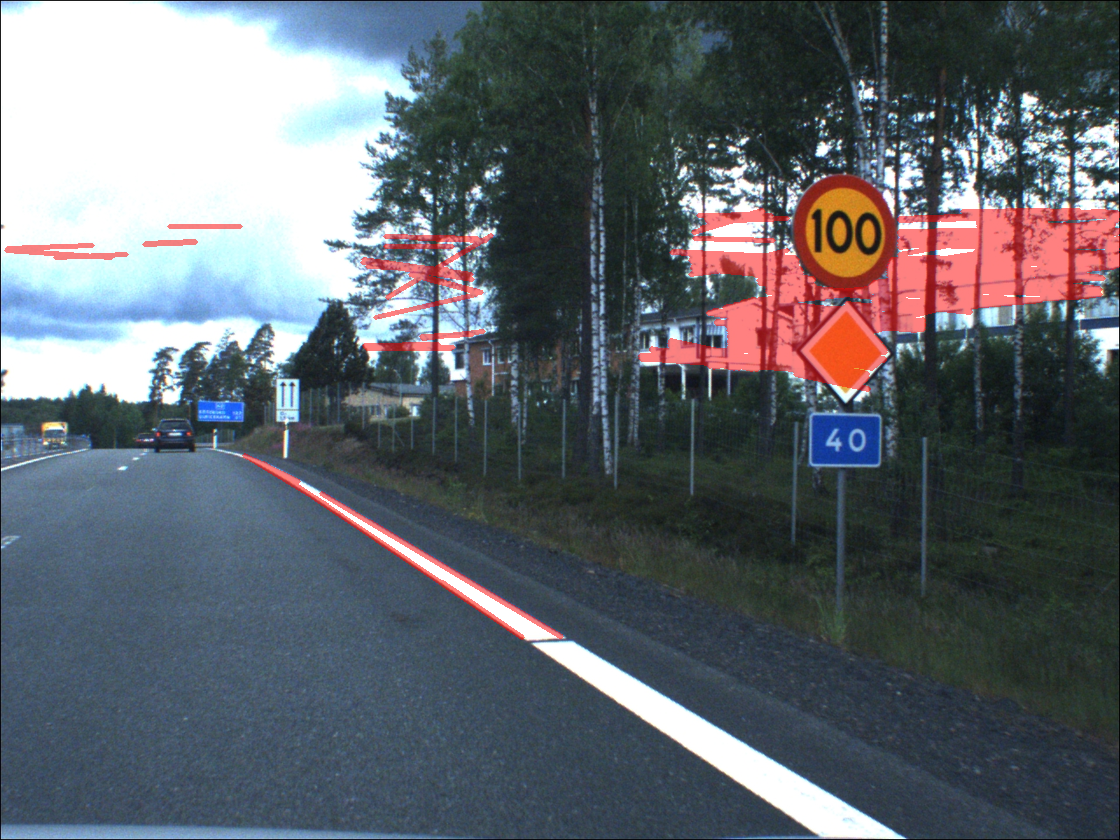
\includegraphics[width = \textwidth]{resources/png/roadbad1.png}
        \end{figure}
        \vspace{-1.3em}
        \begin{figure}
            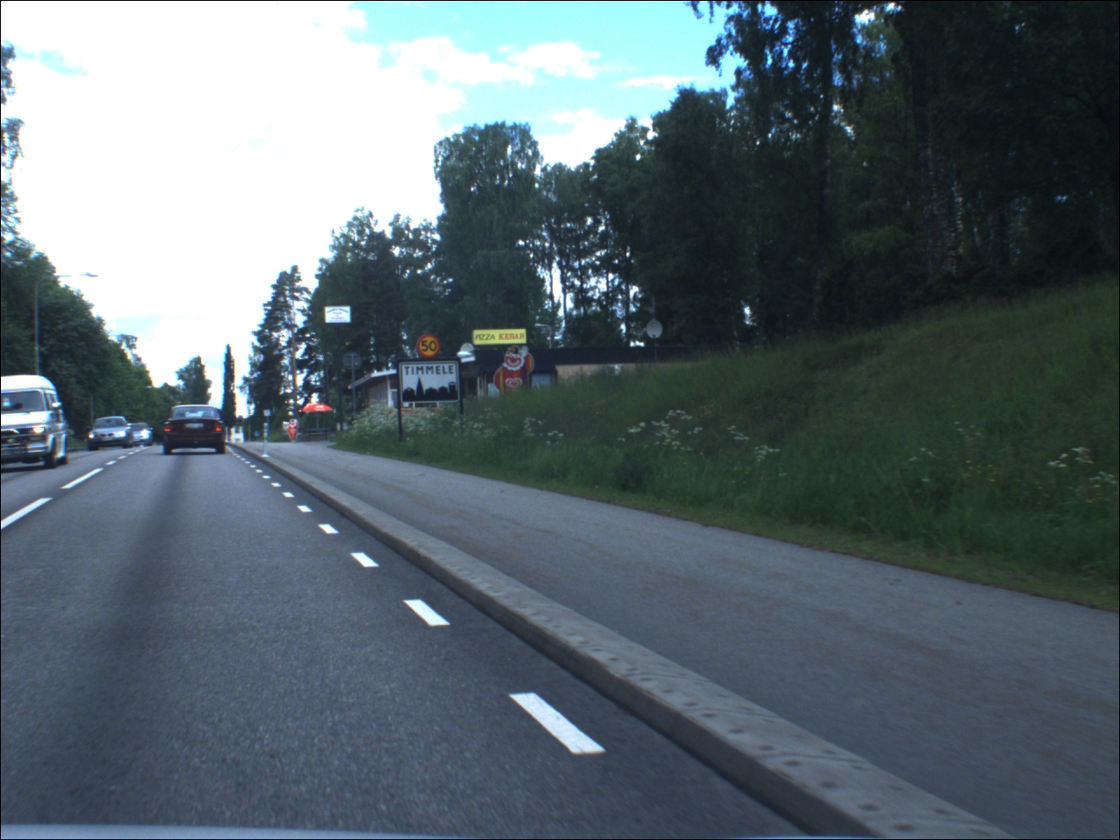
\includegraphics[width = \textwidth]{resources/png/roadbad2.png}
        \end{figure}
        \column{0.45\textwidth}
        \begin{figure}
            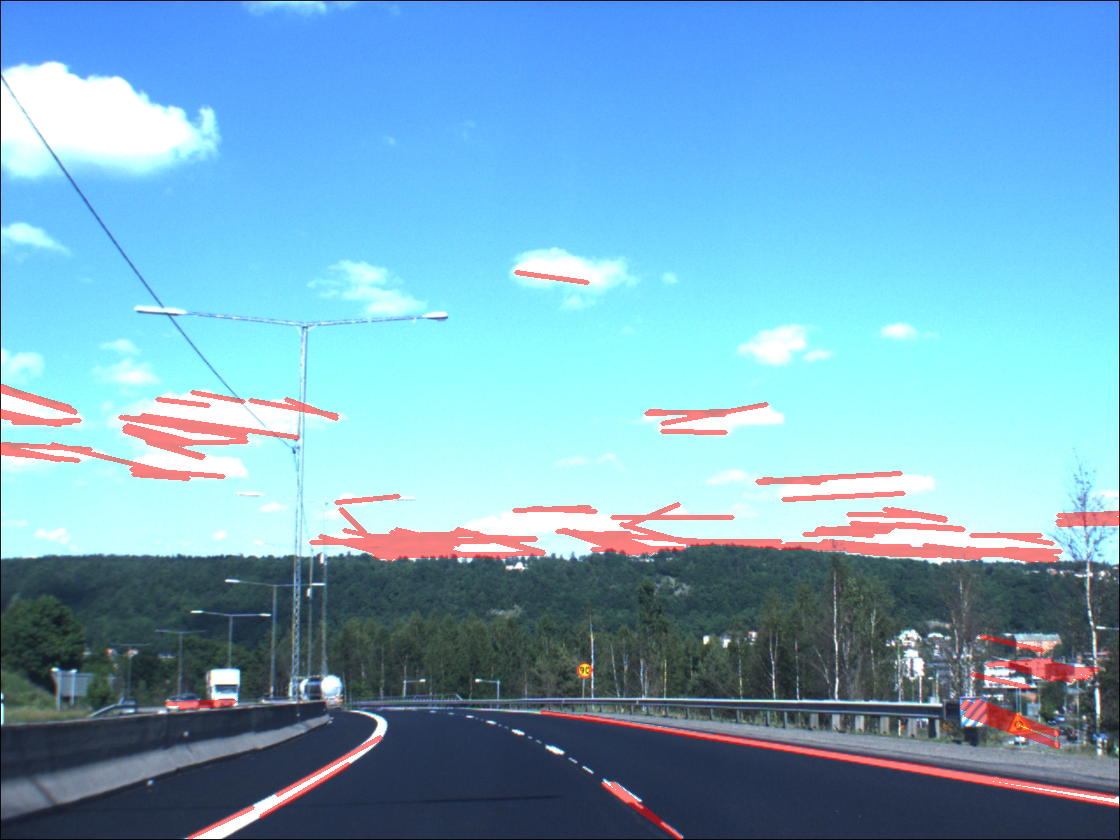
\includegraphics[width = \textwidth]{resources/png/roadbad3.png}
        \end{figure}
        \vspace{-1.3em}
        \begin{figure}
            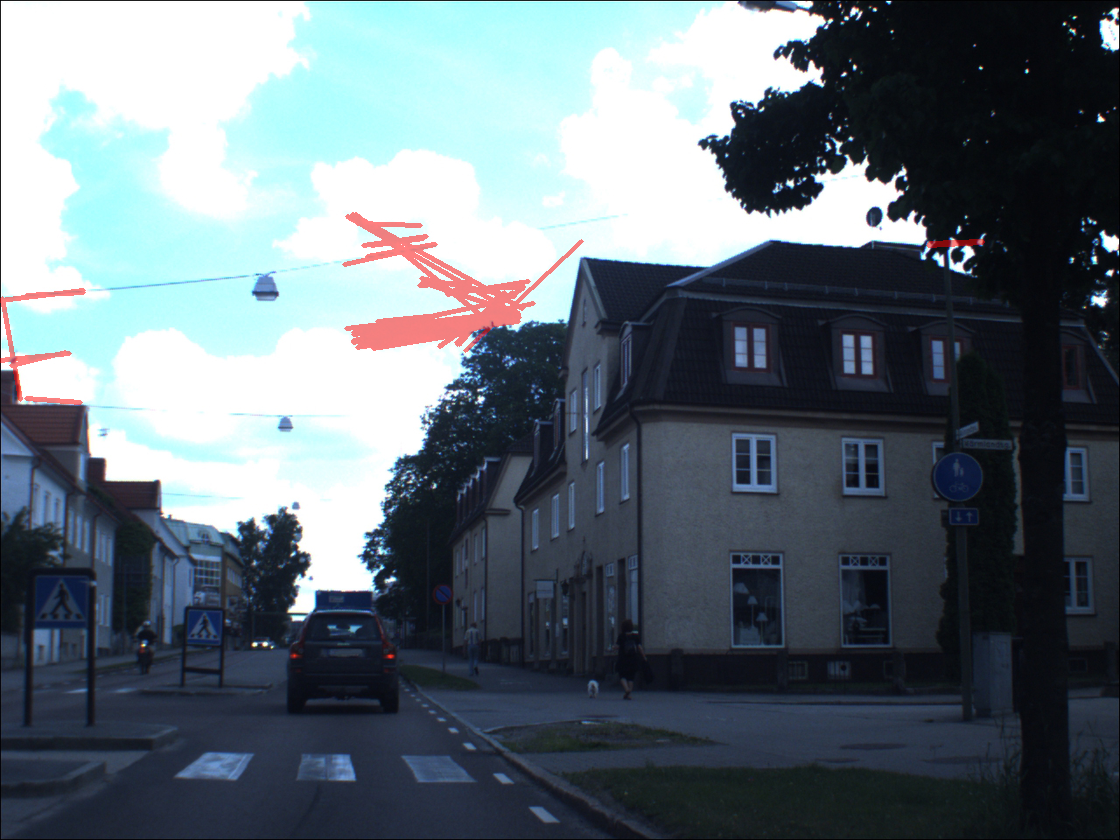
\includegraphics[width = \textwidth]{resources/png/roadbad4.png}
        \end{figure}
    \end{columns}
\end{frame}

\begin{frame}{Road discussion}
Why we had worse results than with the other classes :
    \begin{itemize}
        \item Images are more diverse
        \item Camera angle not standardized
        \item Lanes may curve
        \item Faded lines
        \item Overexposure
        \item ...
    \end{itemize}
\end{frame}

\begin{frame}{Road discussion}
How to get better results ? $\longrightarrow$ Acquisition step ! (not possible here)
    \begin{itemize}
        \item[$\rightarrow$] Standardized angle and position of the camera
        \item[$\rightarrow$] Region of Interest
        \item[$\rightarrow$] Tweak the parameters better
    \end{itemize}
\end{frame}

% ----- Other types of images ----- %
\section{Other types of images}

\begin{frame}{Building as soccer}
    \begin{figure}
        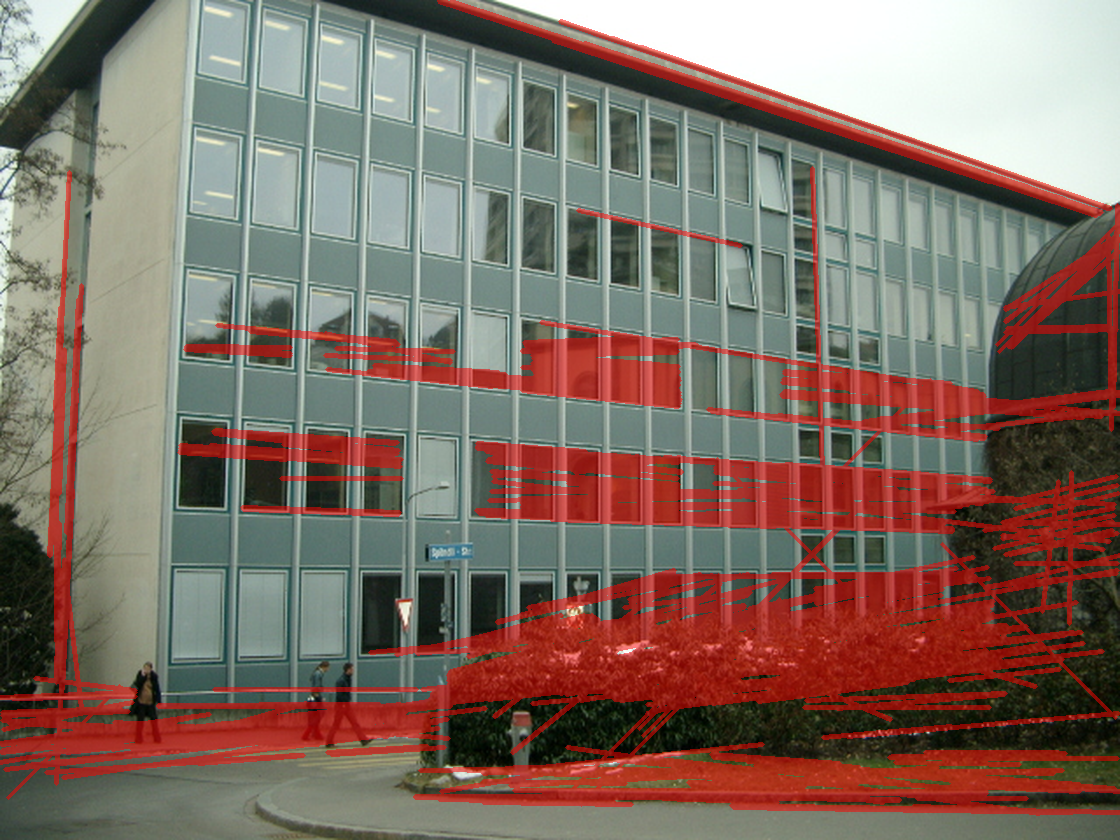
\includegraphics[width=0.9\textwidth]{resources/png/building_as_soccer.png}
    \end{figure}
\end{frame}

\begin{frame}{PCB as road}
    \begin{figure}
        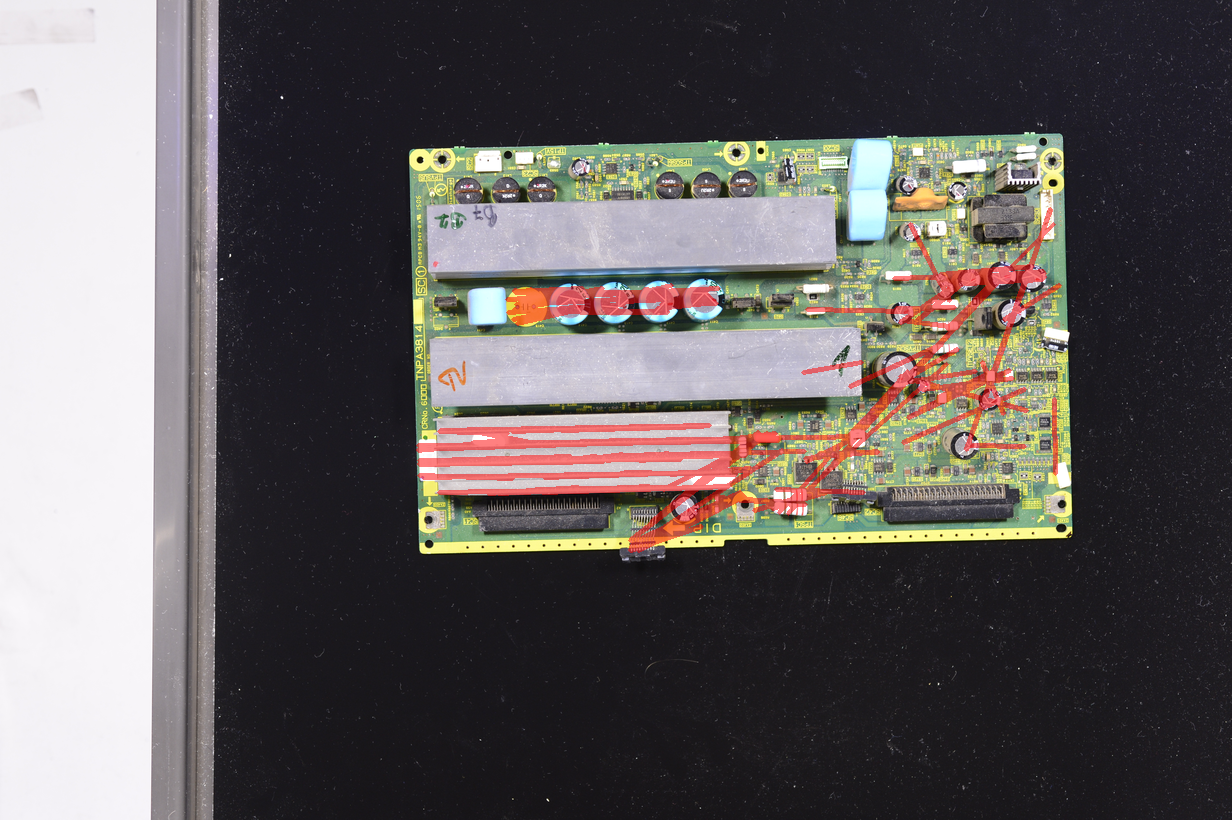
\includegraphics[width=\textwidth]{resources/png/pcb_as_road.png}
    \end{figure}
\end{frame}

\begin{frame}{Building as sudoku}
    \begin{figure}
        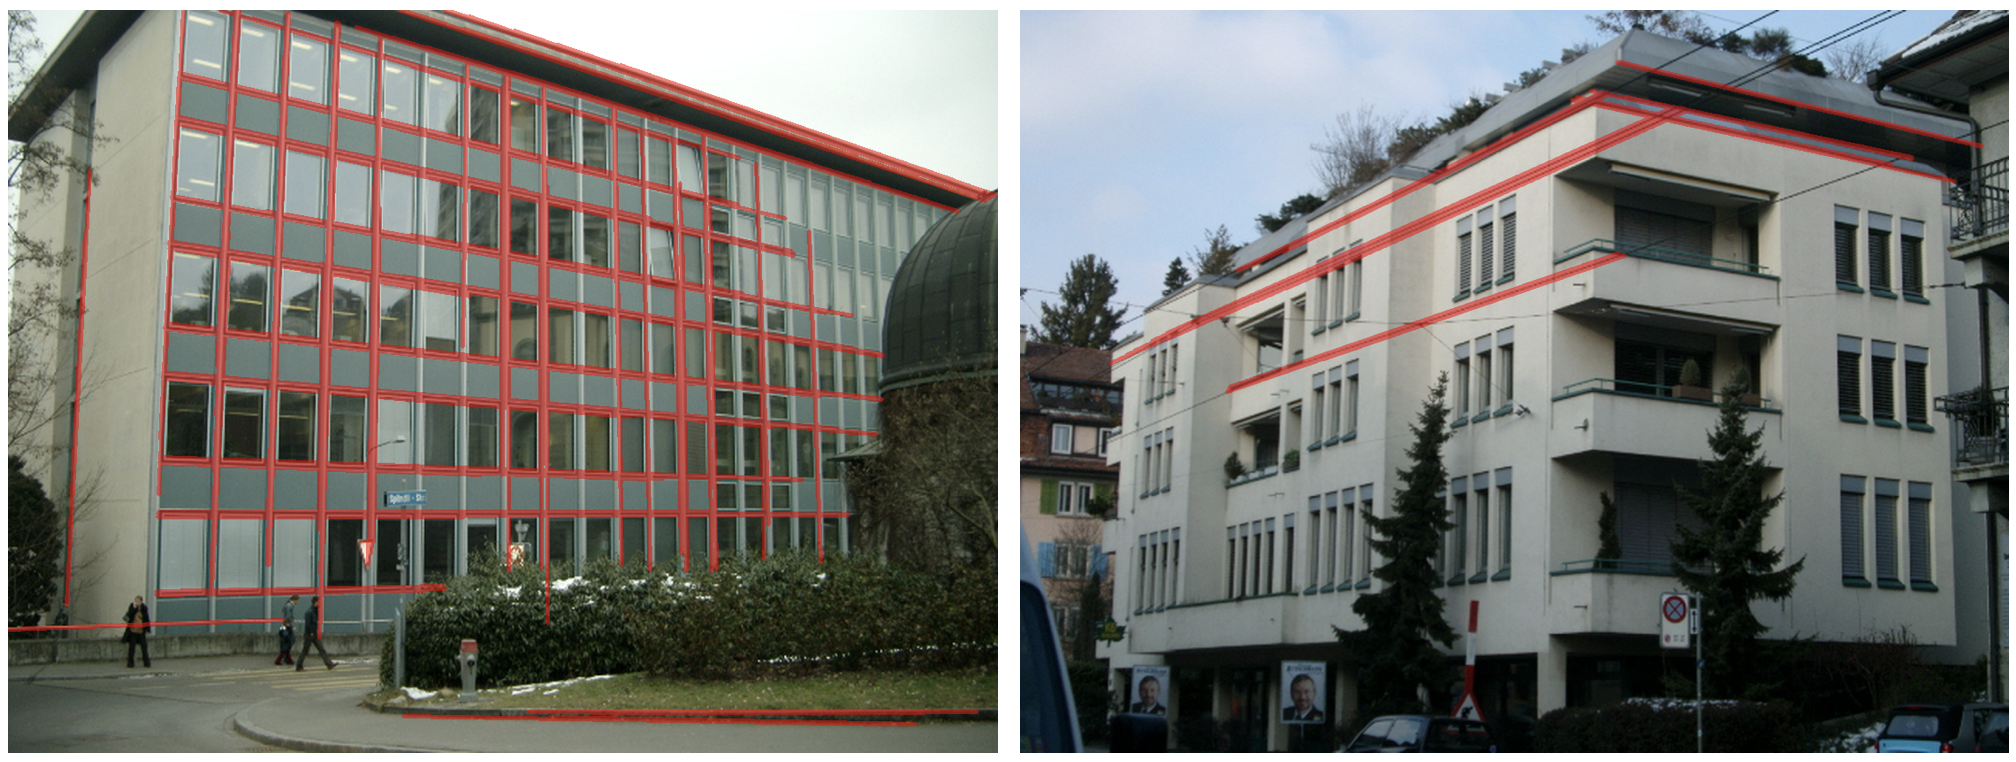
\includegraphics[width=\textwidth]{resources/png/building_as_sudoku.png}
    \end{figure}
    \visible<2->{Sudoku's class is suitable for \textcolor{mLightGreen}{grid-like} objects.}
\end{frame}

\begin{frame}{PCB as sudoku}
    \begin{figure}
        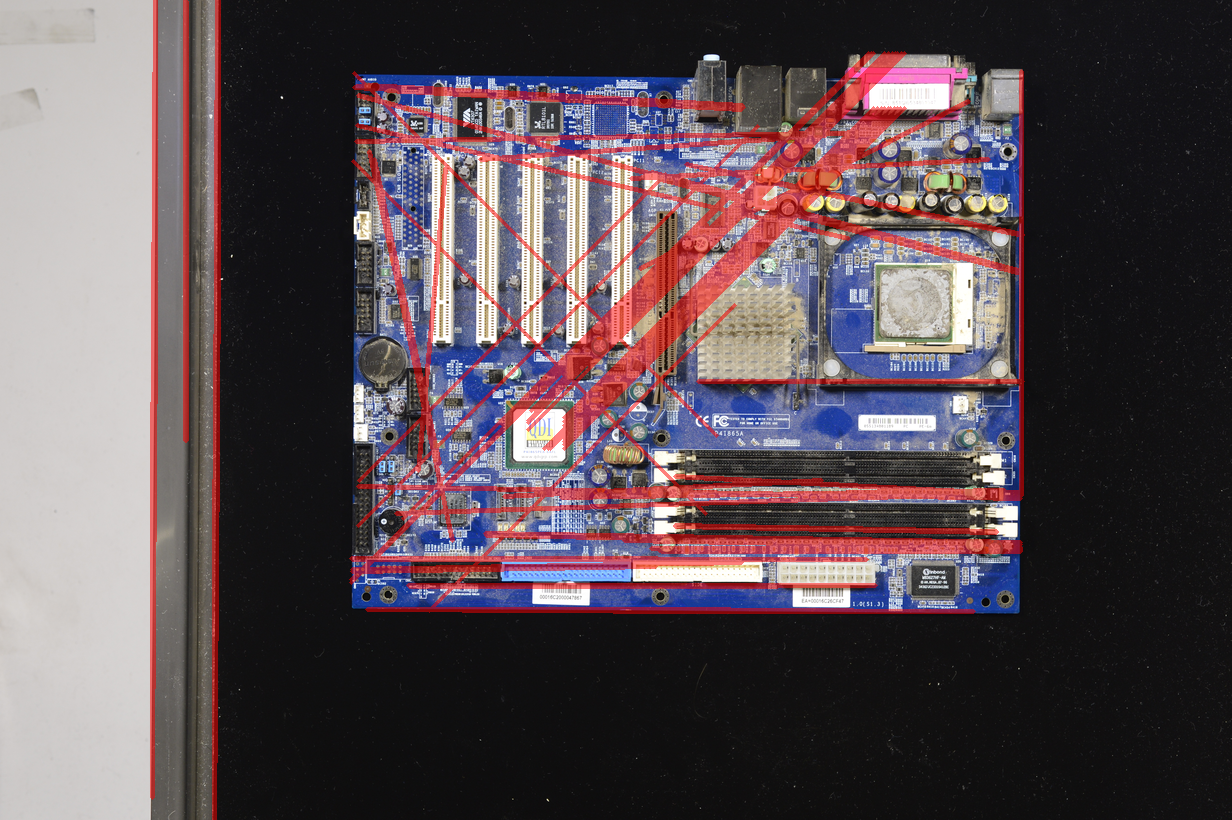
\includegraphics[width=\textwidth]{resources/png/pcb_as_sudoku.png}
    \end{figure}
\end{frame}

% ----- Conclusion ----- %
\section{Conclusion}

\begin{frame}
    \vspace{2em}
    \begin{quote}
        There is no perfect algorithm, only acceptable solutions for particular problems.
    \end{quote}
\end{frame}

% ----- Demonstration ----- %
\begin{frame}[standout]
    Demonstrations
\end{frame}

\end{document}
